\chapter{Lógica matemática}

\section*{Introducción}

Este capítulo introduce los principios y reglas de la lógica matemática, una disciplina que permite analizar argumentos, deducir conclusiones y establecer conexiones entre proposiciones. Se estudian los conceptos de proposición, operadores lógicos (conjunción, disyunción, negación, implicación, bicondicional), tablas de verdad y equivalencias lógicas.
Se analizan las tautologías y contradicciones, proposiciones compuestas que siempre son verdaderas o siempre son falsas, respectivamente. Se introduce la lógica predicativa, una extensión de la lógica proposicional que permite expresar relaciones entre objetos y cuantificar sobre ellos utilizando cuantificadores universales y existenciales.
Finalmente, se presenta el sistema axiomático de Peano, un conjunto de axiomas que permite construir formalmente los números naturales y demostrar teoremas básicos de la aritmética, como el principio de inducción matemática.

\subsection*{Relevancia en ingeniería}

\begin{itemize}
	\item \textit{Diseño de circuitos digitales}: La lógica matemática es la base del diseño de circuitos digitales, donde se utilizan compuertas lógicas para implementar funciones booleanas.
	\item \textit{Verificación y validación de software}: Para demostrar la corrección de programas y sistemas.
	\item \textit{Inteligencia artificial}: La lógica matemática es una herramienta fundamental en la inteligencia artificial, especialmente en áreas como el razonamiento automático y la representación del conocimiento.
	\item \textit{Sistemas de control}: Se aplica en el diseño de sistemas de control para puentes y estructuras, garantizando respuestas adecuadas ante diferentes condiciones.
\end{itemize}

\section{Lógica proposicional}
\index{lógica!proposicional}
\subsection{Proposiciones}
\vspace{1em}
\begin{fmd-definition}[Proposición] \index{proposición}
	Una \gls{proposicion} es una oración que puede ser verdadera o falsa.
\end{fmd-definition}

\begin{fmd-example}
	\begin{itemize}
		\item Proposiciones verdaderas
		\begin{itemize}
			\item El sol sale por el este.
			\item 2 + 2 = 4
			\item La Tierra gira alrededor del Sol.
		\end{itemize}
		
		\item Proposiciones falsas
		\begin{itemize}
			\item Los unicornios existen
			\item 1 + 1 = 3
			\item La luna está hecha de queso verde
		\end{itemize}
	\end{itemize}
\end{fmd-example}

Ahora, veamos ejemplos de oraciones que \textbf{no son proposiciones}:

\begin{fmd-example}
	\begin{itemize}
		\item Preguntas:
		\begin{itemize}
			\item ?`Cómo estás hoy?
			\item ?`Qué hora es?
			\item ?`Dónde está mi libro?
		\end{itemize}
		
		\item Mandatos u Órdenes:
		\begin{itemize}
			\item !`Cerrá la puerta!
			\item Estudiá para el examen.
			\item Limpiá tu habitación.
		\end{itemize}
		
		\item Expresiones abiertas o incompletas:
		\begin{itemize}
			\item $x + 3 = 7$ (no es una proposición completa sin asignar un valor a $x$).
			\item ``Alguien ganará el premio'' (no especifica quién ganará el premio).
		\end{itemize}
	\end{itemize}
\end{fmd-example}

Las proposiciones se representan mediante letras (como $p$, $q$, $r$) y se combinan para formar argumentos más complejos.

\subsection{Operadores lógicos} \label{sec:operadores_logicos}
\index{operador!lógico}
A continuación presentamos varios \glspl{operadorlogico} y sus correspondientes \gls{tablav}. En una tabla de verdad se evalúan todos los posibles valores de verdad de las proposiciones componentes y se determina el valor de verdad resultante de la proposición completa. \index{tabla!verdad}

\subsubsection{Negación $\neg$} \index{negación}
La \gls{negacion} de una proposición $p$ se denota como $\neg p$ o $\sim p$. Representa la idea de que algo no es verdadero. Por ejemplo, si $p$ es ``llueve'', entonces $\neg p$ sería ``no llueve'', tabla \ref{tab:negacion}.

\begin{table}[h]
	\centering
	\begin{tabular}{|c|c|}
		\hline
		$p$ & $\neg p$\\ \hline
		$V$ & $F$ \\ 
		$F$ & $V$ \\ \hline
	\end{tabular}
	\caption{Tabla de verdad de la negación.}
	\label{tab:negacion}
\end{table}

La operación de negación ($\neg$) es análoga a la complementación ($^c$) de la teoría de conjuntos. El paralelismo se construye al considerar la pertenencia de un conjunto como una proposición $p$, si un elemento pertenece a $A$, $p$ es verdadero. El complemento $A^c$ contiene todos los elementos que no pertenecen a $A$, entonces $p$ es falso, por lo tanto $\neg p$ es verdadero, fig. \ref{fig:negacion}.

\begin{figure}[h]
	\centering
	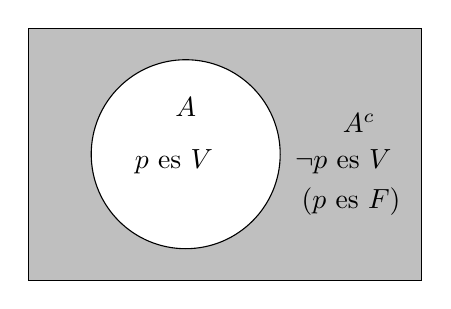
\begin{tikzpicture}[scale=1]
		\filldraw[fill=lightgray] (0, 0) rectangle (5,3.2); % Rectángulo del universo
		\filldraw[fill=white] (2, 1.6) circle (1.2); % Dibuja y rellena el conjunto A
		
		\node at (2, 2.2) {$A$}; % Etiqueta el conjunto A
		\node at (1.85, 1.5) {$p$ es $V$};
		\node at (4.2, 2) {$A^c$}; % Etiqueta el complemento de A
		\node at (4, 1.5) {$\neg p$ es $V$};
		\node at (4.1, 1) {($p$ es $F$)};
	\end{tikzpicture}
	\caption{\(A^c\) es equivalente a $\neg p$}
	\label{fig:negacion}
\end{figure}

\subsubsection{Conjunción \glsentrysymbol{conjuncion}} \index{conjunción}
La \gls{conjuncion} de dos proposiciones $p$ y $q$ se denota como $p \land q$. Representa la idea de que ambas proposiciones son verdaderas. Por ejemplo, si $p$ es ``es lunes'' y $q$ es ``tengo una reunión'', entonces $p \land q$ sería ``es lunes y tengo una reunión''. Su tabla de verdad se muestra en la tabla \ref{tab:conjuncion}.

\begin{table}[H]
	\centering
	\begin{tabular}{|c|c|c|}
		\hline
		$p$ & $q$ & $p \land q$ \\
		\hline
		$V$ & $V$ & $V$ \\
		$V$ & $F$ & $F$ \\
		$F$ & $V$ & $F$ \\
		$F$ & $F$ & $F$ \\
		\hline
	\end{tabular}
	\caption{Tabla de verdad de la conjunción.}
	\label{tab:conjuncion}
\end{table}

La operación lógica de conjunción es análoga a la intersección de la teoría de conjuntos. La intersección $A \cap B$ contiene solo los elementos que pertenecen a $A$ y a $B$ ($p \land q$ es $V$), fig. \ref{fig:conjuncion}.

\begin{figure}[h]
	\centering
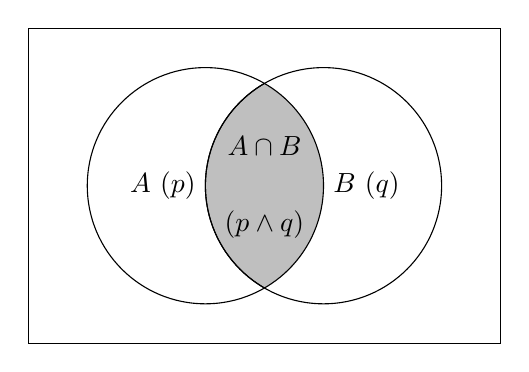
\begin{tikzpicture}
	% Dibujar el universal
	\draw (-3, -2) rectangle (3, 2);
	
	% Sombrear la intersección A ∩ B
	\begin{scope}
		\clip (-.75,0) circle (1.5cm);
		\filldraw[fill=lightgray, draw=black] (.75,0) circle (1.5cm);
	\end{scope}
	
	% Dibujar el conjunto A
	\draw (-.75,0) circle (1.5cm) node[left] {\(A \ (p) \)};
	
	% Dibujar el conjunto B
	\draw (.75,0) circle (1.5cm) node[right] {\(B \ (q)\)};
	
	% Etiqueta de la intersección
	\node at (0, .5) {\(A \cap B\)};
	\node at (0, -.5) {\((p \land q)\)};
\end{tikzpicture}
\caption{$A \cap B$ equivalente a $p \land q$}
\label{fig:conjuncion}
\end{figure}

\subsubsection{Disyunción inclusiva \glsentrysymbol{disyuncion}} \index{disyunción!inclusiva}
La \gls{disyuncion} de dos proposiciones $p$ y $q$ se denota como $p \lor q$. Representa la idea de que al menos una de las proposiciones es verdadera. Por ejemplo, si $p$ es ``estudiaré'' y $q$ es ``veré una película'', entonces $p \lor q$ sería ``estudiaré o veré una película'', tabla \ref{tab:disyuncion}.

\begin{table}[H]
	\centering
	\begin{tabular}{|c|c|c|} \hline
		 $p$ & $q$ & $p$ $\lor q$ \\ \hline
		 $V$ & $V$ & $V$ \\
		 $V$ & $F$ & $V$ \\
		 $F$ & $V$ & $V$ \\
		 $F$ & $F$ & $F$ \\ \hline
	\end{tabular}
	\caption{Tabla de verdad de la disyunción.}
	\label{tab:disyuncion}
\end{table}

La operación lógica de disyunción es análoga a la unión de la teoría de conjuntos. La unión $A \cup B$ contiene los elementos que pertenecen a $A$ o a $B$ o a ambos, en otras palabras, siempre y cuando un elemento pertenezca a $A$ o a $B$ o a ambos $p \lor q$ será $V$, fig. \ref{fig:disyuncion}.

\begin{figure}[H]
	\centering
	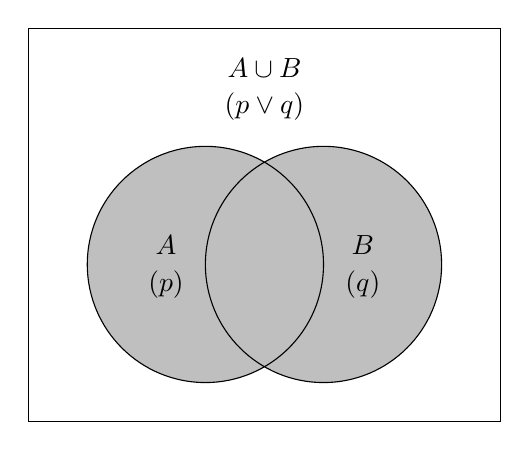
\begin{tikzpicture}
		% Dibujar el universal
		\draw (-3, -2) rectangle (3, 3);
		
		% Sombrear la unión A ∪ B
		\begin{scope}
			\fill[lightgray] (-.75,0) circle (1.5cm);
			\fill[lightgray] (.75,0) circle (1.5cm);
		\end{scope}
		
		% Dibujar el conjunto A
		\draw (-.75,0) circle (1.5cm);
		\node at (-1.25, .25) {\(A\)};
		\node at (-1.25, -.25) {$(p)$};
		
		% Dibujar el conjunto B
		\draw (.75,0) circle (1.5cm);
		\node at (1.25, .25) {\(B\)};
		\node at (1.25, -.25) {$(q)$};
		
		% Etiqueta de la unión
		\node at (0, 2.5) {\(A \cup B\)};
		\node at (0, 2) {\((p \lor q)\)};
	\end{tikzpicture}
	\caption{$A \cup B$ equivalente a $p \lor q$}
	\label{fig:disyuncion}
\end{figure}

\subsubsection{Diferencia simétrica o disyunción excluyente $\oplus$}
\index{diferencia!simétrica} \index{disyunción!excluyente}
La diferencia simétrica o \gls{disyuncione} es verdadera cuando \textit{exactamente una} de las dos proposiciones es verdadera, por ejemplo ``$p$ o $q$ pero no ambos''. Se denota por $p \oplus q$ o $p \nleftrightarrow q$ o $p \underline{\vee} q$, tabla \ref{tab:disyuncion_excluyente}.

\begin{table}[H]
	\centering
	\begin{tabular}{|c|c|c|} \hline
		$p$ & $q$ & $p \oplus q$ \\ \hline
		$V$ & $V$ & $F$ \\
		$V$ & $F$ & $V$ \\
		$F$ & $V$ & $V$ \\
		$F$ & $F$ & $F$ \\ \hline
	\end{tabular}
	\caption{Tabla de verdad de la disyunción excluyente.}
	\label{tab:disyuncion_excluyente}
\end{table}

\begin{fmd-example}[Disyunción excluyente]
	\begin{itemize}
		\item ``Podés elegir té $(p)$ o café $(q)$'' (implícitamente excluyente, ya que normalmente no se consumen ambas bebidas al mismo tiempo). 
		\item ``El interruptor está encendido $(p)$ o apagado $(q)$'' (excluyente, ya que un interruptor solo puede estar en uno de esos dos estados).
		\item ``Ganará la final el equipo local $(p)$ o el equipo visitante $(q)$'' (excluyente, ya que solo uno de los dos equipos puede ganar la final).
	\end{itemize}
\end{fmd-example}

Esta operación es análoga a la diferencia simétrica de la teoría de conjuntos. $A \triangle B$ contiene los elementos que pertenecen a $A$ o a $B$ pero no a ambos, fig. \ref{fig:disyuncion_excluyente}.

\begin{figure}[h]
	\centering
	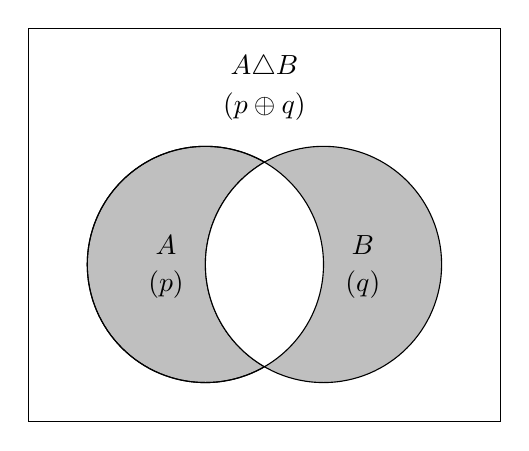
\begin{tikzpicture}
		% Dibujar el universal
		\draw (-3, -2) rectangle (3, 3);
		
		% Sombrear la parte de A que no está en B
		\filldraw[fill=lightgray, draw=black] (-.75,0) circle (1.5cm);
		\begin{scope}
			\clip (.75,0) circle (1.5cm);
			\draw[fill=white] (-.75,0) circle (1.5cm);
		\end{scope}
		
		% Sombrear la parte de B que no está en A
		\filldraw[fill=lightgray, draw=black] (.75,0) circle (1.5cm);
		\begin{scope}
			\clip (-.75,0) circle (1.5cm);
			\draw[fill=white] (.75,0) circle (1.5cm);
		\end{scope}
		
		\draw (-.75, 0) circle (1.5cm);
		
		% Etiquetas de los conjuntos A y B
		\node at (-1.25, .25) {\(A\)};
		\node at (-1.25, -.25) {\((p)\)};
		\node at (1.25, .25) {\(B\)};
		\node at (1.25, -.25) {\((q)\)};
		
		% Etiqueta de la diferencia simétrica
		\node at (0, 2.5) {\(A \triangle B\)};
		\node at (0, 2) {\((p \oplus q)\)};
	\end{tikzpicture}
	\caption{$A \triangle B$ equivalente a $p \oplus q$}
	\label{fig:disyuncion_excluyente}
\end{figure}


\subsubsection{Implicación o condicional $\implies$} \index{implicación} \index{condicional}
Si se combinan dos proposiciones por medio de las palabras \textit{``si..., entonces...''} se obtiene un \gls{implicacion} o \textit{proposición condicional}. La implicación de una proposición $p$ a otra $q$ se denota como $p \implies q$. Representa la idea de que si $p$ es verdadero, entonces $q$ también debe serlo. Por ejemplo, si $p$ es ``estudiaré'', entonces $q$ es ``aprobaré el examen''. La tabla de verdad es:

\begin{table}[H]
	\centering
	\begin{tabular}{|c|c|c|} \hline
		$p$ & $q$ & $p \implies q$ \\ \hline
		$V$ & $V$ & $V$ \\
		$V$ & $F$ & $F$ \\
		$F$ & $V$ & $V$ \\
		$F$ & $F$ & $V$ \\ \hline
	\end{tabular}
	\caption{Tabla de verdad de la implicación}
	\label{tab:implicacion}
\end{table}

Se observa que $p \implies q$ es verdadero si y sólo si no se da el caso de que $p$ sea verdadero y $q$ falso.

En teoría de conjuntos la inclusión $A \subset B$ es verdadero si y sólo si no existe un elemento que esté en $A$ pero no en $B$. La conexión entre la implicación lógica y la inclusión de conjuntos se visualiza en la fig. \ref{fig:inclusion_logica}.

\begin{figure}[H]
	\centering
	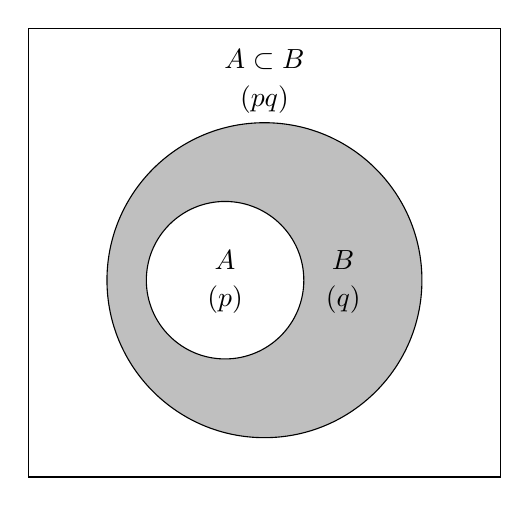
\begin{tikzpicture}
		% Dibujar el universal
		\draw (-3, -2.5) rectangle (3, 3.2);
		
		% Dibujar el conjunto B
		\filldraw[fill=lightgray, draw=black] (0,0) circle (2cm);
		\node at (1, .25) {$B$};
		\node at (1, -.25) {$(q)$};
		
		% Dibujar el conjunto A dentro de B
		\filldraw[fill=white, draw=black] (-0.5,0) circle (1cm);
		\node at (-.5, .25) {$A$};
		\node at (-.5, -.25) {$(p)$};
		
		% Etiqueta de la implicación e inclusión
		\node at (0, 2.8) {\(A \subset B\)};
		\node at (0, 2.3) {\((p \implies q)\)};
	\end{tikzpicture}
	\caption{$A \subset B$ equivalente a $p \implies q$}
	\label{fig:inclusion_logica}
\end{figure}

Proposiciones. Para algún $x \in U$:
\begin{itemize}
	\item $p: x \in A$.
	\item $q: x \in B$.
	\item La implicación $p \implies q$ se interpreta como: Si $x$ está en $A$, entonces $x$ está en $B$.
\end{itemize}

Paralelismo con la tabla de verdad:
\begin{itemize}
	\item $p = V$, $q = V$ $\left(x \in A \land x \in B \right)$: Corresponde a elementos que están tanto en $A$ como en $B$, lo cual es consistente con $A \subset B$, la implicación es verdadera.
	\item $p=V$, $q = F$, $(x \in A \land x \not \in B)$: Este caso viola la inclusión $A \subset B$ ya que hay un elemento en $A$ que no está en $B$, la implicación es falsa.
	\item $p = F$, $q = V$ $(x \not \in A \land x \in B)$: Esto es consistente con $A \subset B$, ya que elementos fuera de $A$ pueden estar en $B$ sin violar la inclusión, la implicación es verdadera.
	\item $p = F$, $q = F$ $\left( x \not \in A \land x \not \in B \right)$: También es consistente con $A \subset B$, ya que elementos que no están en $A$ ni tampoco en $B$ no afectan la inclusión, la implicación es verdadera.
\end{itemize}


\subsubsection{Doble implicación o bicondicional $\iff$} \index{implicación!doble} \index{implicación!condicional} \index{bicondicional} \index{si y solo si} \label{sec:bicondicional}
 La doble implicación, o \gls{bicondicional}, o proposición ``si y solo si'' se denota como $p \iff q$. Representa la idea de que $p$ es verdadero si y solo si $q$ también lo es. Puede verse, si es verdadera, como cumplimiento en ambos sentidos las implicaciones $p \implies q$ y $q \implies b$. Tabla \ref{tab:bicondicional}.

\begin{table}[H]
	\centering
	\begin{tabular}{|c|c|c|} \hline
		$p$ & $q$ & $p \iff q$ \\ \hline
		$V$ & $V$ & $V$ \\
		$V$ & $F$ & $F$ \\
		$F$ & $V$ & $F$ \\
		$F$ & $F$ & $V$ \\ \hline
	\end{tabular}
	\caption{Tabla de verdad de la bicondicional}
	\label{tab:bicondicional}
\end{table}

\begin{fmd-example}
	Si $p$ es ``Es fin de semana'' y $q$ es ``No tengo clases''.
	\begin{itemize}
		\item La implicación $p \implies q$ sería: ``Es un fin de semana entonces no tengo clases''.
		\item La implicación recíproca $q \implies p$ sería: ``No tengo clases entonces es un fin de semana''
		\item La bicondicional $p \iff q$ sería: ``Es fin de semana si y solo si no tengo clases''
	\end{itemize}
\end{fmd-example}

En la teoría de conjuntos, su equivalente es la \textbf{igualdad de conjuntos}. Si definimos, igual que antes, $p$: pertenencia al conjunto $A$ y $q$: pertenencia al conjunto $B$, la doble implicación $p \iff q$ se interpreta como: un elemento está en A si y solo si está en B.

\subsection{Condiciones necesarias y suficientes}
\index{condición!necesaria} \index{condición!suficiente}
\subsubsection{Condición necesaria y condición suficiente}

Consideremos la tabla de verdad de la implicación, tabla \ref{tab:implicacion}, que, reescribimos a continuación:

\begin{table}[H]
	\centering
	\begin{tabular}{|c|c|c|} \hline
		$p$ & $q$ & $p \implies q$ \\ \hline
		$V$ & $V$ & $V$ \\
		$V$ & $F$ & $F$ \\
		$F$ & $V$ & $V$ \\
		$F$ & $F$ & $V$ \\ \hline
	\end{tabular}
\end{table}

Hay tres casos en que $p \implies q$ es $V$, y entre ellos hay uno en que $p$ es $V$, en el cual resulta $q$ verdadera. Es obvio que nos referimos al primer renglón de la tabla, y se tiene que si $p \implies q$ es $V$ y $p$ es $V$, entonces $q$ es $V$. Se dice entonces que en antecedente $p$ es \textit{condición suficiente} para el consecuente $q$.

En cambio, si $p$ es $F$, nada podemos decir de $q$, puesto que puede ser $V$ o $F$, por otra parte, cuando $p \implies q$ es $V$, si $q$ es $V$, entonces $p$ puede ser $V$ o $F$; mas, para que $p$ sea $V$ se necesita que $q$ lo sea. Se dice entonces que $q$ es \textit{condición necesaria} para $p$.

Resumiendo, si $p \implies q$ es $V$, entonces $p$ es condición suficiente para $q$ y $q$ es condición necesaria para $p$, suele expresarse así:

\begin{itemize}
	\item $q$ si $p$: condición suficiente;
	\item $p$ sólo si $q$: condición necesaria.
\end{itemize}

\begin{fmd-example}
	``Si $T$ es equilátero, entonces $T$ es isósceles''
	
	En este caso:
	\begin{itemize}
		\item $p$: $T$ es equilátero;
		\item $q$: $T$ es isósceles.
	\end{itemize}
	
	$p$ es condición suficiente para $q$, en este ejemplo, que un triángulo sea equilátero es suficiente para asegurar que sea isósceles. Por otra parte, $T$ es equilátero sólo si es isósceles; es decir, que un triángulo sea isósceles es necesario para que sea equilátero.
\end{fmd-example}

\subsubsection{Condición necesaria y suficiente}

Sea ahora la doble implicación $p \iff q$, esto significa $(p \implies q) \land (q \implies p)$. Si $p \iff q$ es $V$, entonces $p \implies q$ es $V$ y $q \implies p$, es $V$. Se tiene, atendiendo a la primera, que $p$ es condición suficiente para $q$; y, teniendo en cuenta la segunda implicación, ocurre que $p$ es condición necesaria para $q$.

Si $p \implies q$ es $V$, entonces el antecedente $p$ es condición necesaria y suficiente para el consecuente $q$.

Análogamente, en el caso de la doble implicación verdadera, el consecuente $q$ es también condición necesaria y suficiente para el antecedente $p$.

\begin{fmd-example}
	``$T$ es equilátero si y sólo si $T$ es equiángulo''
	
	Es la doble implicación de las proposiciones:
	\begin{itemize}
		\item $p$: $T$ es equilátero;
		\item $q$: $T$ es equiángulo.
	\end{itemize}
	Aquella es $V$, y cualquiera de las dos proposiciones es condición necesaria y suficiente de la otra.
\end{fmd-example}

\subsection{Tautología, contradicción y contingencia}

\subsubsection{Tautología} \index{tautología}
\vspace{1em}
\begin{fmd-definition}[Tautología]
	Cuando una proposición compuesta, como por ejemplo $(p \implies q) \land p \implies q$ es verdadera, independientemente de los valores de verdad de las proposiciones componentes, se dice que tal proposición es una \gls{tautologia} o \textit{ley lógica}, o sea, una tautología es una proposición lógica que siempre es verdadera.
\end{fmd-definition}

En el cálculo proposicional se utilizan las siguientes leyes o tautologías cuyas demostraciones se reduce a la confección de las correspondientes tablas de verdad.

\begin{enumerate}
	\item \textbf{Identidad}
	\[ p \implies p; \qquad p \iff p \]
	
	\[ p \land \mbox{verdadero} = p \quad \mbox{y} \quad p \lor \mbox{falso} = p \]
	
	\item \textbf{Ley del tercero excluido}
	\[ p \lor \neg p = V\]
	Una proposición es verdadera o su negación es verdadera.
	
	\item \textbf{No contradicción}
	\[ p \land \neg p = F \]
	
	\item \textbf{Involución o doble negación}
	\[ \neg (\neg p) \iff p \]
	La doble negación es equivalente a una afirmación: ``no, no $p$, equivale a $p$''
	\item Idempotencia
	\[ (p \land p) \iff p \quad y \quad (p \lor p) \iff p\]
	\item \textbf{Conmutatividad}
	\begin{enumerate}[label=\alph*)]
		\item De la conjunción: $p \land q \iff q \land p$. 		
		\item De la disyunción: $p \lor q \iff q \lor p$.
	\end{enumerate}
	\item \textbf{Asociatividad}
	\begin{enumerate}[label=\alph*)]
		\item De la conjunción: $(p \land q) \land r \iff p \land (q \land r)$,
		
		\item De la disyunción: $(p \lor q) \lor r \iff p \lor (q \lor r)$
	\end{enumerate}
	\item \textbf{Distributividad}
	\begin{enumerate}[label=\alph*)]
		\item De la conjunción respecto de la disyunción:
		\[ p \lor (q \land r) \iff (p \land r) \lor (q \land r) \]
		
		\item De la disyunción respecto de la conjunción:
		\[(p \land (q \lor r) \iff (p \lor r) \land (q \lor r) \]
		
		\item De la implicación respecto de la disyunción
		\[ \left( p \implies q \lor r \right) \iff \left( (p \implies q) \lor (p \implies r) \right) \]

		\item De la implicación respecto de la conjunción
		\[ \left( p \implies q \land r \right) \iff \left( (p \implies q) \land (p \implies r) \right) \]
	\end{enumerate}
	\item \textbf{Leyes de De Morgan}
	\begin{enumerate}[label=\alph*)]
		\item La negación de una disyunción es equivalente a la conjunción de las negaciones:
		\[ \neg (p \lor q) \iff \neg p \land \neg q\]
		\item La negación de  una conjunción es equivalente a la disyunción de las negaciones.
		\[ \neg (p \land q) \iff \neg p \lor \neg q \]
	\end{enumerate}
	
	\item \textbf{Leyes de absorción total}
	\begin{enumerate}
		\item Primera forma: \[ p \lor (p \land q) \iff p \]
		\item Segunda forma: \[ p \land (p \lor q) \iff p \]
	\end{enumerate}
	Si $p$ es verdadero (o falso) ambos miembros son verdaderos (o falsos) independientemente de $q$.
	
	\item \textbf{Leyes de absorción parcial}
	\begin{enumerate}
		\item \( p \lor \left(\neg p \land q\right) \iff p \lor q \)
		\item \( p \land \left(\neg p \lor q\right) \iff p \land q \)
	\end{enumerate}
\end{enumerate}

La mayoría de estas leyes lógicas tienen sus análogas en teoría de conjuntos, algunas de las cuales se listan en la tabla \ref{tab:logica_conjuntos}.

\begin{table}[H]
	\centering
	\small
	\begin{tabular}{|l|c|c|}
		\hline
		\textbf{Ley} & \textbf{Lógica} & \textbf{Conjuntos} \\ \hline
		Identidad & \makecell{ \( p \implies p \) \\ \( p \iff p \) \\ \( p \land \text{V} = p \) \\ \( p \lor \text{F} = p \)} & \makecell{ \(A = A\) \\ \\ \( A \cap U = A \) \\ \( A \cup \emptyset = A \)} \\ \hline
		Tercero excluido & \( p \lor \neg p = \text{V} \) & \( A \cup A^c = U \) \\ \hline
		No contradicción & \( p \land \neg p = \text{F} \) & \( A \cap A^c = \emptyset \) \\ \hline
		Involución & \( \neg(\neg p) \iff p \) & \( \left(A^c\right)^c = A \) \\ \hline
		Idempotencia & \makecell{ \( p \land p \iff p \) \\ \( p \lor p \iff p \)} & \makecell{ \( A \cap A = A \) \\ \( A \cup A = A \)} \\ \hline
		Conmutatividad & \makecell{\( p \land q \iff q \land p \) \\ \( p \lor q \iff q \lor p \)} & \makecell{\( A \cap B = B \cap A \) \\ \( A \cup B = B \cup A \)} \\ \hline
		Asociatividad & \makecell{ \( (p \land q) \land r \iff p \land (q \land r) \) \\ \( (p \lor q) \lor r \iff p \lor (q \lor r) \)} & \makecell{\( (A \cap B) \cap C = A \cap (B \cap C) \) \\ \( (A \cup B) \cup C = A \cup (B \cup C) \)} \\ \hline
		Distributividad & \makecell{\( p \land (q \lor r) \iff (p \land q) \lor (p \land r) \) \\ \( p \lor (q \land r) \iff (p \lor q) \land (p \lor r) \)} & \makecell{\( A \cap (B \cup C) = (A \cap B) \cup (A \cap C) \) \\ \( A \cup (B \cap C) = (A \cup B) \cap (A \cup C) \)} \\ \hline
		Leyes de De Morgan & \makecell{ \( \neg(p \lor q) \iff \neg p \land \neg q \) \\ \( \neg(p \land q) \iff \neg p \lor \neg q \)} & \makecell{\( (A \cup B)^c = A^c \cap B^c \) \\ \( (A \cap B)^c = A^c \cup B^c \)} \\ \hline
		Ley de absorción & \makecell{\( p \lor (p \land q) \iff p \) \\ \( p \land (p \lor q) \iff p \)} & \makecell{\( A \cup (A \cap B) = A \) \\ \( A \cap (A \cup B) = A \)} \\ \hline
	\end{tabular}
	\caption{Paralelismo entre las leyes lógicas y las de conjuntos.}
	\label{tab:logica_conjuntos}
\end{table}

\subsubsection{Contradicción}
\index{contradicción}
Una \gls{contradiccion} es una proposición lógica que siempre es falsa, sin importar los valores de verdad de sus componentes. Es una fórmula que es falsa en todas las interpretaciones posibles.

\begin{fmd-example}[Contradicción]
	\begin{itemize}
		\item Conjunción de una proposición y su negación:
		\[ p \land \neg p \]
		
		\item Negación de una tautología:
		\[ \neg \left( p \lor \neg p \right) \]
	\end{itemize}
\end{fmd-example}

\subsubsection{Contingencia} \index{contingencia}
Una \gls{contingencia} es una proposición que puede ser tanto verdadera como falsa, dependiendo de las circunstancias. Su valor de verdad depende de la situación o el contexto.

\begin{fmd-example}[Contingencia]
	\begin{itemize}
		\item \textbf{Afirmaciones sobre el futuro}: ``\textit{Lloverá mañana en Caaguazú}''. Esta afirmación es contingente porque depende de factores meteorológicos que aún no se han determinado.
		\item \textbf{Juicios de valor}: ``\textit{La pizza es más rica que la pasta}''. Esta afirmación es contingente porque depende de las preferencias personales de cada individuo.
		\item \textbf{Hipótesis científicas}: ``\textit{La materia oscura existe}''. Aunque hay evidencia que la apoya, aún no se ha probado de manera concluyente, por lo que es una afirmación contingente.
		\item \textbf{Eventos históricos}: ``\textit{La Segunda Guerra Mundial comenzó en 1939}''. Esta afirmación es contingente en el sentido de que pudo haber ocurrido de otra manera si diferentes factores históricos hubieran sido distintos.
	\end{itemize}
\end{fmd-example}

\textbf{?`Qué hace a una proposición contingente?}

\begin{enumerate}
	\item \textit{Dependencia del contexto}: Su valor de verdad depende completamente de las circunstancias específicas en las que se evalúa.
	\item \textit{Posibilidad y necesidad}: Una contingencia es posible (puede ser verdadera) y al mismo tiempo, es posible que no sea verdadera (puede ser falsa).
	\item \textit{No es una verdad necesaria}: A diferencia de las tautologías, las contingencias no son verdades universales que se mantienen en todos los mundos posibles.
	\item \textit{No es una falsedad necesaria}: Tampoco son falsedades absolutas como las contradicciones.
\end{enumerate}

\subsection{Funciones booleanas}
En lógica simbólica, las \textit{funciones booleanas} son aquellas que toman uno o más valores de verdad (verdadero o falso) como entrada y producen un único valor de verdad como salida. Estas funciones se construyen utilizando operadores lógicos homónimos, que son:

\begin{itemize}
	\item \textbf{Conjunción} (AND): Representada por $\land$ o $\cdot$. Es verdadera solo si ambas proposiciones de entrada son verdaderas.
	\item \textbf{Disyunción} (OR): Representada por $\lor$ o $+$. Es verdadera si al menos una de las proposiciones de entrada es verdadera.
	\item \textbf{Negación} (NOT): Representada por $\neg$ o una barra sobre la proposición. Invierte el valor de verdad de la proposición.
\end{itemize}

A partir de estos operadores básicos, podemos construir funciones booleanas más complejas. Algunas de las funciones booleanas más comunes son:

\begin{enumerate}
	\item \textbf{Función Identidad}:
	\begin{itemize}
		\item Definición: La salida es igual a la entrada.
		\item Expresión: $f(p) = p$
		\item Ejemplos:
		\begin{enumerate}
			\item Si $p$ es verdadero, entonces $f(p)$ es verdadero.
			\item Si $p$ es falso, entonces $f(p)$ es falso.
		\end{enumerate}
	\end{itemize}
	
	\item \textbf{Función Constante}:
	\begin{itemize}
		\item Definición: La salida siempre es el mismo valor de verdad, independientemente de la entrada.
		\item Expresión:
		\begin{itemize}
			\item $f(p) = 1$ (Función constante verdadera)
			\item $f(p) = 0$ (Función constante falsa)
		\end{itemize}
		\item Ejemplos:
		\begin{enumerate}
			\item Si $p$ es verdadero, $f(p)$ sigue siendo verdadero (para la función constante verdadera) o falso (para la función constante falsa).
			\item Si $p$ es falso, $f(p)$ sigue siendo verdadero (para la función constante verdadera) o falso (para la función constante falsa).
		\end{enumerate}
	\end{itemize}
	
	\item \textbf{Función Negación}:
	\begin{itemize}
		\item Definición: La salida es la negación de la entrada.
		\item Expresión: \( f(p) = \neg p \)
		\item Ejemplos:
		\begin{enumerate}
			\item Si $p$ es verdadero, entonces $f(p)$ es falso.
			\item Si $p$ es falso, entonces $f(p)$ es verdadero.
		\end{enumerate}
	\end{itemize}
	
	\item \textbf{Función Conjunción}:
	\begin{itemize}
		\item Definición: La salida es verdadera solo si todas las entradas son verdaderas.
		\item Expresión: \( f(p, q) = p \land q \)
		\item Ejemplos:
		\begin{enumerate}
			\item Si $p$ es verdadero y $q$ es verdadero, entonces $f(p, q)$ es verdadero.
			\item Si $p$ es verdadero y $q$ es falso, o viceversa, o ambos son falsos, entonces $f(p, q)$ es falso.
		\end{enumerate}
	\end{itemize}
	
	\item \textbf{Función Disyunción}:
	\begin{itemize}
		\item Definición: La salida es verdadera si al menos una de las entradas es verdadera.
		\item Expresión: \( f(p, q) = p \lor q \)
		\item Ejemplos:
		\begin{enumerate}
			\item Si $p$ es verdadero o $q$ es verdadero, o ambos son verdaderos, entonces $f(p, q)$ es verdadero.
			\item Si $p$ es falso y $q$ es falso, entonces $f(p, q)$ es falso.
		\end{enumerate}
	\end{itemize}
	
	\item \textbf{Función Implicación}:
	\begin{itemize}
		\item Definición: La salida es falsa solo si la primera entrada es verdadera y la segunda es falsa
		\item Expresión: \( f(p, q) = p \implies q  \)
		\item Ejemplos:
		\begin{enumerate}
			\item Si $p$ es verdadero y $q$ es verdadero, entonces $f(p, q)$ es verdadero.
			\item Si $p$ es verdadero y $q$ es falso, entonces $f(p, q)$ es falso.
			\item Si $p$ es falso, independientemente del valor de $q$, $f(p, q)$ es verdadero
		\end{enumerate}
	\end{itemize}
	
	\item \textbf{Función Equivalencia} (Bicondicional):
	\begin{itemize}
		\item Definición: La salida es verdadera si ambas entradas tienen el mismo valor de verdad
		\item Expresión: \( f(p, q) = p \iff q  \)
		\item Ejemplos:
		\begin{enumerate}
			\item Si $p$ es verdadero y $q$ es verdadero, o si $p$ es falso y $q$ es falso, entonces $f(p, q)$ es verdadero.
			\item Si $p$ es verdadero y $q$ es falso, o viceversa, entonces $f(p, q)$ es falso.
		\end{enumerate}
	\end{itemize}
\end{enumerate}

\subsection{Proposiciones equivalentes}
\index{proposición!equivalente}
Al unir dos proposiciones cualesquiera por medio de la frase \textit{``si y sólo si''} cuyo símbolo\footnote{Sección \ref{sec:bicondicional}, pág. \pageref{sec:bicondicional}.} es \( \iff \)) se obtiene una proposición compuesta que se llama \textit{equivalencia}. Las proposiciones conectadas de esta manera reciben los nombres de \textit{miembro izquierdo} y \textit{miembro derecho} de la equivalencia. Al afirmar la equivalencia de las proposiciones, se excluye la posibilidad de que una sea verdadera y la otra falsa; por lo tanto, una equivalencia es verdadera si sus miembros izquierdo y derecho son o bien ambos verdaderos o bien ambos falsos; en caso contrario la equivalencia es falsa.

Dos proposiciones son \textit{equivalentes} si y solo si tienen el mismo valor de verdad en todas las posibles combinaciones de valores de verdad de sus proposiciones componentes. En otras palabras, sus tablas de verdad son idénticas.

La equivalencia lógica captura la idea de que dos proposiciones, aunque expresadas de manera diferente, representan la misma información desde el punto de vista lógico. Si dos proposiciones son equivalentes, podemos sustituir una por la otra en cualquier contexto lógico sin alterar el significado o la validez del razonamiento.

\begin{fmd-example}[Proposiciones equivalentes]
	Dada la proposición compuesta:
	\begin{center}
		\emph{``$x$ es un número positivo si, y solo si, $3x$ es un número positivo''}
	\end{center}
	
	De \textit{$x$ es un número positivo} ($p$) se sigue que \textit{$3x$ es un número positivo} ($q$), (en símbolos $p \implies q$) y, recíprocamente, de \textit{$3x$ es un número positivo} se sigue que \textit{$x$ es un número positivo} ($q \implies p$). Las condiciones de que $x$ sea un número positivo y que $3x$ sea un número positivo son equivalentes entre sí ($p \iff q$).
	
	La condición de ser $x$ un número positivo es \textit{necesaria y suficiente} para que $3x$ sea un número positivo, recíprocamente, para que $x$ sea un número positivo es necesario y suficiente que $3x$ lo sea, significa que, cada una de las proposiciones representa una \textit{condición necesaria y suficiente} para la otra.
\end{fmd-example}

\subsubsection{Verificación de equivalencia}

La forma más directa de comprobar si dos proposiciones son equivalentes es construir sus tablas de verdad y compararlas. Si las columnas de resultados finales son idénticas, entonces las proposiciones son equivalentes. Utilizaremos el símbolo de equivalencia ``$\equiv$''

\begin{fmd-example}
	Probar la ley de De Morgan: \( \neg \left(p \land q \right) \equiv \neg p \lor \neg q \)
	\begin{table}[H]
		\centering
		\begin{tabular}{|c|c|c|c|c|c|c|}
			\hline
			$p$ & $q$ & $p \land q$ & $\neg (p \land q)$ & $\neg p$ & $\neg q$ & $\neg p \lor \neg q$ \\
			\hline
			V & V & V & F & F & F & F \\
			V & F & F & V & F & V & V \\
			F & V & F & V & V & F & V \\
			F & F & F & V & V & V & V \\
			\hline
		\end{tabular}
	\end{table}
	Se observa que la cuarta columna, de $\neg \left(p \land q \right)$, y la última columna, de \( \neg p \lor \neg q \) son idénticas, por lo tanto estas proposiciones son equivalentes.
\end{fmd-example}

\begin{fmd-example}[Implicación material]
	Probar que: \( p \implies q \equiv \neg p \lor q \)

\begin{table}[H]
	\centering
	\begin{tabular}{|c|c|c|c|c|}
		\hline
		$p$ & $q$ & $p \implies q$ & $\neg p$ & $\neg p$ $\lor q$ \\
		\hline
		V & V & V & F & V \\
		V & F & F & F & F \\
		F & V & V & V & V \\
		F & F & V & V & V \\
		\hline
	\end{tabular}
\end{table}
	Se observa que la tercera columna, de $p \implies q$, y la última columna, de \( \neg p \lor q \) son idénticas, por lo tanto estas proposiciones son equivalentes. Esta equivalencia se conoce como \textit{ley de implicación material}.
	\label{ex:implicacion}
\end{fmd-example}

El concepto de equivalencia lógica es fundamental en la simplificación de expresiones lógicas, en la demostración de teoremas y en la resolución de problemas lógicos. Nos permite manipular y transformar proposiciones manteniendo su significado original, lo que facilita el análisis y la comprensión de argumentos lógicos complejos.

\subsection{Álgebra de proposiciones}
\index{álgebra!proposiciones}
El álgebra de proposiciones nos proporciona un marco formal para combinar y manipular proposiciones utilizando operadores lógicos, lo que nos permite analizar y razonar sobre argumentos y demostraciones de manera rigurosa.

\begin{fmd-example}[Simplificación de expresiones lógicas]
	Simplifica la siguiente expresión lógica utilizando las leyes del álgebra de proposiciones:
	
	\[
	(\neg p \land q) \lor (p \land \neg q) \lor (p \land q)
	\]
	\textbf{Solución}
	\[ \begin{array}{ll}
		(\neg p \land q) \lor (p \land \neg q) \lor (p \land q) & \\
		\equiv (\neg p \land q) \lor [(p \land \neg q) \lor (p \land q)] & \mbox{agrupando términos}\\
		\equiv (\neg p \land q) \lor [p \land (\neg q \lor q)] & \mbox{distributividad}\\
		\equiv (\neg p \land q) \lor p & \mbox{ley del tercero excluido}\\
		\equiv p \lor (\neg p \land q) & \mbox{conmutatividad de la disyunción}\\
		\equiv p \lor q & \mbox{ley de absorción}
		\end{array} \]
\[ (\neg p \land q) \lor (p \land \neg q) \lor (p \land q) \equiv p \lor q \]
\end{fmd-example}

\begin{fmd-example}[Demostración de equivalencia]
	Demuestra que las siguientes expresiones son equivalentes:
	
	\[
	p \implies \left( q \lor r \right) \equiv \left( p \land \neg q \right) \implies r
	\]
	\textbf{Solución}
	\[ \begin{array}{ll}
	p \implies \left( q \lor r \right) & \\
		\equiv \neg p \lor \left(q \lor r\right) & \mbox{implicación material}\\
		\equiv \left(\neg p \lor q \right) \lor r& \mbox{asociatividad}\\
		\equiv \neg \left(p \land \neg q\right) \lor r & \mbox{De Morgan}\\
		\equiv \left(p \land \neg q\right) \implies r & \mbox{implicación material}
	\end{array} \]
\end{fmd-example}

\subsection{Proposiciones condicionales}
\index{proposiciones!condicionales}
Cuando tenemos una proposición en forma de implicación (como $p \implies q$,  ``si $p$, entonces $q$''), podemos derivar tres proposiciones adicionales, estas son la recíproca, la proposición contraria (o la negación de la proposición original) y la proposición contrarrecíproca.

\begin{enumerate}
	\item \textbf{Proposición recíproca} ($q \implies p$): Se forma al \textit{invertir la implicación} de una proposición dada. Ejemplo con el teorema de Pitágoras: \index{proposición!recíproca} \index{recíproca}
	\begin{itemize}
		\item Este teorema establece que: ``en un triángulo rectángulo, la suma de los cuadrados de los catetos es igual al cuadrado de la hipotenusa'' ($p \implies q$).
		
		
		\item La proposición recíproca afirmaría que: ``si la suma de los cuadrados de los catetos es igual al cuadrado de la hipotenusa, entonces el triángulo es rectángulo'' ($q \implies q$).
	\end{itemize}
	
	\item \textbf{Proposición Contraria} ($\neg p \implies \neg q$): \index{proposición!contraria} \index{contraria}
	Se obtiene al reemplazar tanto el antecedente como el consecuente de la proposición original por sus negaciones. Por ejemplo:
	
	\begin{itemize}
		\item Proposición original: ``Si llueve, entonces la calle estará mojada'' ($p \implies q$)
		\item Contraria:``Si no llueve, entonces la calle no estará mojada'' ($\neg p \implies \neg q$).
	\end{itemize}
	
	\item \textbf{Proposición Contrarrecíproca} ($\neg q \implies \neg p$): La contrarrecíproca es el resultado de intercambiar el antecedente y el consecuente en la proposición contraria. Por ejemplo: \index{proposición!contrarrecíproca} \index{contrarrecíproca}
	\begin{itemize}
		\item Proposición original: ``Si estudio, entonces saco buenas notas'' ($p \implies q$)
		\item Proposición contraria: ``Si no estudio, entonces no saco buenas notas'' ($\neg p \implies \neg q$).
		\item Contrarrecíproca: ``Si no saco buenas notas, entonces no estoy estudiando'' ($\neg q \implies \neg p$).
	\end{itemize}
\end{enumerate}

Estas tres proposiciones están relacionadas entre sí y nos ayudan a explorar diferentes aspectos de una implicación. Es importante entenderlas para razonar correctamente en lógica y matemáticas.

\textbf{Resumen}, en símbolos:

\begin{itemize}
	\item Implicación: $p \implies q$
	
	\item Recíproca: $q \implies p$
	
	\item Contraria: $\neg p \implies \neg q$
	
	\item Contrarrecíproca: $\neg q \implies \neg p$
\end{itemize}

Las cuatro implicaciones anteriores se llaman conjugadas, y cualquiera de ellas puede tomarse como directa. El siguiente esquema nos proporciona una relación que las vincula:
\begin{figure}[H]
	\centering
	\begin{tikzpicture}[scale=1]
		\draw (-1.5, .75) rectangle (7.5, -3.75);
		
		\coordinate (A) at (0, 0);
		\coordinate (B) at (6, 0);
		\coordinate (C) at (0, -3);
		\coordinate (D) at (6, -3);
		
		\node at (A) {$p \implies  q$};
		\node at (B) {$q \implies  p$};
		\node at (C) {$\neg p \implies \neg q$};
		\node at (D) {$\neg q \implies \neg p$};
		
		\node at ($(A)!0.5!(B)$) {recíprocos};
		\node at ($(C)!0.5!(D)$) {recíprocos};
		
		\node[rotate=90] at ($(A)!0.5!(C)$) {contrarios};
		\node[rotate=90] at ($(B)!0.5!(D)$) {contrarios};
		
		\node[rotate=-30] at ($(A)!0.55!(D)$) {contra \quad recíprocos};
		\node[rotate=30] at ($(C)!0.55!(B)$) {contra \quad recíprocos};
	\end{tikzpicture}
\end{figure}

Es fácil verificar que las implicaciones contrarrecíprocas son equivalentes, es decir, las siguientes bicondicionales son tautologías:
\[ (p \implies q) \iff (\neg q \implies \neg p) \]
\[ (q \implies p) \iff (\neg p \implies \neg q) \]

Si la implicación directa es $V$, también lo es la contrarrecíproca, y no podemos afirmar la verdad de la recíproca o de la contraria. Pero, si son verdaderos un condicional y su recíproco o contrario, entonces son verdaderos los cuatro, y las proposiciones antecedente y consecuente son equivalentes.

\subsubsection{Demostración matemática}
\index{demostración!matemática}

Consideremos, previamente, los siguientes conceptos:
\begin{itemize}
	\item Decimos que $q$ es un \textit{múltiplo} de $p$ si $\exists n \in \mathbb{N} \ / \ q = np$
	\item También decimos que $n$ y $p$ son \textit{factores} de $q$ o que \textit{dividen} a $q$.
	\item Un elemento $p\in \mathbb{N}$ distinto de 1 se llama \textit{primo} si sus únicos factores son el 1 y el propio $p$.
	\item Dos números enteros son \textit{coprimos} cuando no tienen ningún divisor común positivo aparte del 1.
\end{itemize}


Se presenta continuamente la necesidad de demostrar la verdad de
\[ \begin{array}{c}
	p\\
	\mbox{Hipótesis}
\end{array} \implies \begin{array}{c}
q\\
\mbox{Tesis}
\end{array} \]
y, de acuerdo con lo expuesto, se presentan dos métodos:

\begin{enumerate}[label=\roman*)]
	\item \textit{Directo}: Si $p = F$, nada hay que probar, pues en este caso $p \implies q$ es $V$. Si $p$ es $V$ hay que establecer que el valor de verdad de $q$ es $V$.
	
	\begin{fmd-example}[Demostración por el método directo] \label{ex:directo}
		\textit{Proposición} ($p \Rightarrow q$): Si el cuadrado de un número entero, $a^2$ es múltiplo de un número primo $k$, entonces el número $a$ debe ser también múltiplo de $k$.
		
		\begin{itemize}
			\item Hipótesis ($p$): el cuadrado de un número entero $a^2$ es múltiplo de un número primo $k$;
			\item Tesis ($q$): $a$ es también múltiplo de $k$.
		\end{itemize}
		
		\textit{Demostración}:
		
		Supongamos que $a^2$ es múltiplo de $k$, donde $k$ es un número primo. Entonces, existe un entero $m$ tal que:
		$$a^2 = km$$
		
		La factorización única en números primos\footnote{Teorema \ref{teo:aritmetica} fundamental de la aritmética, pág. \pageref{teo:aritmetica}} nos dice que todo número entero se puede expresar de forma única como un producto de números primos (despreciando el orden de los factores). 
		
		Si descomponemos $a$ en sus factores primos, tendremos:
		$$a = p_1^{e_1}p_2^{e_2}...p_n^{e_n}$$
		donde $p_1, p_2, ..., p_n$ son números primos y $e_1, e_2, ..., e_n$ son números enteros no negativos.
		
		Elevando al cuadrado ambos lados de la igualdad, obtenemos:
		$$a^2 = p_1^{2e_1}p_2^{2e_2}...p_n^{2e_n}$$
		
		Como $a^2 = km$, entonces la factorización prima de $a^2$ debe contener el factor primo $k$ con alguna multiplicidad. Pero como la factorización prima es única, esto implica que $k$ debe ser igual a uno de los primos $p_1, p_2, ..., p_n$.
		
		Por lo tanto, $k$ divide a $a$, es decir, $a$ es múltiplo de $k$.
	\end{fmd-example}
	
	
	
	\item \textit{Indirecto}:
	\begin{enumerate}[label=\alph*)]
		\item Se utiliza la \textit{contrarrecíproca}, esto es, demostrar la verdad de $p \implies q$ es equivalente a probar la verdad de $\neg q \implies \neg p$.
		
		\begin{fmd-example}[Demostración por contrarrecíproca]
	\textit{Proposición} ($ p \Rightarrow q$): Si un número entero es par, entonces su cuadrado también es par.
	
	\begin{itemize}
		\item Hipótesis ($p$): Un número entero es par;
		\item Tesis ($q$):  su cuadrado también es par
	\end{itemize}
	
	\textit{Demostración}:
	
			La contrarrecíproca ($\neg q \Rightarrow \neg p$) es: Si el cuadrado de un número entero no es par (es decir, es impar), entonces el número entero tampoco es par (es impar).
			
			Supongamos que $n$ es el número entero del que estamos hablando,  y que $n^2$ es impar ($\neg q$). Si esto es así, entonces $n^2 = 2k + 1$ para algún entero $k$.
			
			Supongamos ahora que $n$ es par ($p$). Entonces $n = 2m$ para algún entero $m$. 
			Elevando al cuadrado ambos lados, obtenemos:
			\[ n^2 = (2m)^2 = 4 m^2 = 2 (2m)^2 \]
			
			Esto implica que $n^2$ es par, lo cual contradice nuestra suposición inicial de que $n^2$ era impar.
			
			Por lo tanto, nuestra suposición de que $n$ es par debe ser falsa. Concluimos que si $n^2$ es impar ($\neg q$), entonces $n$ también debe ser impar ($\neg p$).
			
			Hemos demostrado la contrarecíproca del teorema original, lo que implica que el teorema original también es verdadero.
		\end{fmd-example}
		
		
		\item Por \textit{contradicción} o \textit{reducción al absurdo}:
		\begin{enumerate}
			\item Se supone que la tesis ($q$) es falsa, con lo cual, se parte del caso $p = V$ y $q = F$;
			\item Se derivan otras afirmaciones utilizando reglas lógicas;
			\item Si se llega a una contradicción (por ejemplo $q \land \neg q = V$), se concluye que $q = V$.
		\end{enumerate}
		\begin{fmd-example}[Demostración por reducción al absurdo]
			\textit{Proposición}: Existen infinitos números primos.
			
			\textit{Demostración de Euclides}:
			
			Supongamos lo contrario, es decir, que existe un número finito de números primos. Llamémoslos $p_1, p_2, ..., p_n$. Consideremos el número:
			$$q = p_1p_2...p_n + 1$$
			
			Este número $q$ no es divisible por ninguno de los números primos $p_1, p_2, ..., p_n$, ya que al dividir $q$ entre cualquiera de estos números siempre obtendremos un resto de 1. 
			
			Si $q$ es primo, entonces hemos encontrado un nuevo número primo que no estaba en nuestra lista original, lo que contradice nuestra suposición inicial. Si $q$ no es primo, entonces debe tener un factor primo. Pero este factor primo no puede ser ninguno de los $p_1, p_2, ..., p_n$, ya que hemos demostrado que $q$ no es divisible por ninguno de ellos. Nuevamente, esto contradice nuestra suposición inicial.
			
			En ambos casos llegamos a una contradicción, lo que demuestra que nuestra suposición inicial era falsa. Por lo tanto, debe haber infinitos números primos.
		\end{fmd-example}
	\end{enumerate}
\end{enumerate}

\begin{lgnote}
También se tiene el \textit{método de inducción} del que se hablará en la sección \ref{sec:induccion}, pág. \pageref{sec:induccion}.
\end{lgnote}

\begin{fmd-example}[Irracionalidad de $\sqrt{3}$ por reducción al absurdo]
\textit{Proposición}: $\sqrt{3}$ es un número irracional.

\textit{Demostración}:

Supongamos lo contrario, es decir, que $\sqrt{3}$ es racional. Entonces, existen dos números enteros coprimos $a$ y $b$ tales que:
$$\sqrt{3} = \frac{a}{b}$$
Elevando al cuadrado ambos lados de la igualdad, obtenemos:
$$3 = \frac{a^2}{b^2}$$
Lo cual implica que $a^2 = 3b^2$.

De esta última igualdad, podemos concluir que $a^2$ es un múltiplo de 3. Si el cuadrado de un número es múltiplo de 3, entonces el número también debe ser múltiplo de 3 (ejemplo \ref{ex:directo}). Por lo tanto, podemos escribir $a = 3k$, donde $k$ es un entero. Sustituyendo en la ecuación anterior:
$$(3k)^2 = 3b^2$$
$$9k^2 = 3b^2$$
$$3k^2 = b^2$$

Ahora vemos que $b^2$ también es múltiplo de 3, lo que implica que $b$ también es múltiplo de 3.

Hemos llegado a una contradicción: asumimos al principio que $a$ y $b$ eran coprimos (es decir, no tenían factores comunes excepto 1), pero acabamos de demostrar que ambos son múltiplos de 3, lo que significa que tienen un factor común de 3. 

Esta contradicción demuestra que nuestra suposición inicial era falsa. Por lo tanto, $\sqrt{3}$ no puede ser racional y debe ser irracional.
\end{fmd-example}

\subsubsection{Negación de una implicación} \index{negación!implicación}
Las proposiciones $p \implies q$ y $\neg (p \land \neg q)$ son equivalentes, por implicación material y ley de De Morgan:
\[ p \implies q \equiv \neg p \lor q \equiv \neg \left( p \land \neg q \right) \]

En consecuencia, la negación de la primera equivale a la negación de la segunda, es decir:
\[ \neg (p \implies q) \iff \neg [ \neg (p \land \neg q)] \]

y por la propiedad de \textit{involución} se tiene:
\[ \neg (p \implies q) \iff (p \land \neg q) \]

La negación de una implicación no es una implicación, sino la conjunción del antecedente con la negación del consecuente.

\begin{fmd-example}[Negación de una implicación \(\neg (p \implies q) \iff (p \land \neg q)  \)]
	Sean las implicaciones:
	
	\begin{enumerate}[label=\roman*)]
		\item Si hoy es lunes ($p$), entonces mañana es miércoles ($q$).
		
		Cuya negación es: ``Hoy es lunes ($p$) y mañana no es miércoles ($\neg q$)''
		
		\item ``Si estudias para el examen ($p$), entonces obtendrás una buena calificación ($q$)''
		
		La negación de esta afirmación sería: ``Estudias para el examen ($p$), pero no obtienes una buena calificación ($\neg q$)''
		
		\item ``Si un número es divisible por 4, entonces también es divisible por 2'' ($p \implies q$).
		
		La negación es: ``Hay un número que es divisible por 4, pero no es divisible por 2'' ($ p \land \neg q$).
	\end{enumerate}
\end{fmd-example}

\subsection{Argumento y razonamiento deductivo válido}

\subsubsection{Argumento} \index{argumento}
\begin{fmd-definition}[Argumento]
	Un \gls{argumento} es una secuencia de proposiciones (llamadas premisas) que pretende respaldar o justificar una proposición final (llamada conclusión). Un argumento se presenta usualmente de la siguiente forma:
	\[ p_1, p_2, \dots, p_n \implies q \]
	
	\begin{itemize}[itemsep=-3pt]
		\item $p_1$: premisa 1
		\item $p_2$: premisa 2
		\item $\qquad \vdots$
		\item $p_n$: premisa $n$
		\item Por lo tanto, $q$: conclusión.
	\end{itemize}
\end{fmd-definition}

\subsubsection{Razonamiento deductivo válido}
\vspace{1em} \index{razonamiento!válido}
\begin{fmd-definition}
	Un argumento se considera un \gls{razonamiento} si, y solo si, es imposible que todas sus premisas sean verdaderas y su conclusión sea falsa. En otras palabras, la verdad de las premisas garantiza la verdad de la conclusión. La validez de un argumento depende únicamente de su forma lógica, no del contenido específico de las proposiciones.
\end{fmd-definition}

El razonamiento deductivo válido es un proceso lógico en el que, a partir de premisas o afirmaciones, se llega a una conclusión de manera irrefutable. Un razonamiento es válido si la conclusión sigue necesariamente de las premisas, siguiendo las reglas de la lógica.

Por ejemplo:
\[ \frac{\begin{array}{l}
		p \implies  q\\
		p
\end{array}}{q} \]

Si tenemos las premisas $(p \Rightarrow q)$ y $(p)$, entonces la conclusión $(q)$ es válida. Esta es la ley del \textit{modus!ponens} de la que se hablará más en la pág. \pageref{def:ponens}.

\subsubsection{Relación entre argumento y razonamiento deductivo válido}

Un argumento puede ser válido o inválido. Un argumento válido es aquel en el que la conclusión se sigue necesariamente de las premisas, de esta manera, representa un razonamiento deductivo válido. Por otro lado, un argumento inválido es aquel en el que la conclusión no se sigue lógicamente de las premisas, incluso si las premisas son verdaderas.


\begin{fmd-example}[Argumento válido] \index{argumento!válido}
	\[ \frac{\begin{array}{l}
			p \implies  q\\
			p
	\end{array}}{q} \]
	\begin{itemize}
		\item \textit{Premisa 1}: Si llueve, entonces la calle está mojada (\( p \implies q \)).
		\item \textit{Premisa 2}: Está lloviendo ($p$)
		\item \textit{Conclusión}: Por lo tanto, la calle está mojada ($q$).
	\end{itemize}
	Este argumento es válido porque si las dos premisas son verdaderas, la conclusión también debe ser verdadera.
\end{fmd-example}

\begin{fmd-example}[Argumento inválido] \index{argumento!inválido}
	\[ \frac{\begin{array}{l}
			p \implies  q\\
			q
	\end{array}}{p} \]
	\begin{itemize}
		\item \textit{Premisa 1}: Si llueve, entonces la calle está mojada ($p \implies q$)
		\item \textit{Premisa 2}: La calle está mojada ($q$).
		\item \textit{Conclusión}: Por lo tanto, está lloviendo ($p$).
	\end{itemize}
	Este argumento es inválido porque la calle podría estar mojada por otras razones además de la lluvia. Aunque las premisas sean verdaderas, la conclusión no se sigue necesariamente de ellas.
\end{fmd-example}

El razonamiento deductivo válido es esencial en la lógica matemática y en muchas otras disciplinas, ya que nos permite construir argumentos sólidos y confiables. Al utilizar argumentos válidos, podemos estar seguros de que si nuestras premisas son verdaderas, nuestra conclusión también lo será.

\subsection{Reglas de Inferencia}
\index{reglas!inferencia}
Las \gls{reglasinferencia} son patrones lógicos fundamentales que nos permiten deducir nuevas proposiciones a partir de un conjunto de proposiciones dadas (premisas). Son herramientas esenciales en la construcción de argumentos válidos y en la demostración de teoremas en lógica matemática.

Son como las reglas de un juego. El juego se juega con proposiciones o fórmulas lógicas. Se empieza con conjuntos de fórmulas que se denominan \textit{premisas}. El objeto del juego es utilizar las reglas de inferencia de manera que conduzcan a otras fórmulas que se denominan \textit{conclusiones}. El paso lógico de las premisas a la conclusión es una \textit{deducción}.\vspace{3mm}

La conclusión que se obtiene se dice que es una \textit{consecuencia lógica} de las premisas si cada paso que se da para llegar a la conclusión está permitido por una regla.\vspace{3mm}

La idea de inferencia es: \textit{de premisas verdaderas se obtienen sólo conclusiones verdaderas}.

\textbf{Características}:

\begin{itemize}
	\item \textit{Validez}: Una regla de inferencia es válida si, siempre que las premisas sean verdaderas, la conclusión deducida también es verdadera.
	\item \textit{Forma lógica}: Las reglas de inferencia se basan en la forma lógica de las proposiciones, no en su contenido específico. Esto significa que se pueden aplicar a cualquier conjunto de proposiciones que tengan la misma estructura lógica, independientemente de su significado.
	\item \textit{Deducción}: Las reglas de inferencia nos permiten realizar deducciones, esto es, pasar de proposiciones conocidas a nuevas proposiciones que se siguen lógicamente de ellas.
\end{itemize}


\begin{enumerate}[label=\alph*)]
	\item Ley del \textbf{modus ponens}: \label{def:ponens} \index{modus!ponens}
	\[ p \implies q, \ p \ \vdash \ q \]
	Donde:
	\begin{itemize}
		\item $\vdash$ denota la relación de inferencia lógica (``se deduce'').
	\end{itemize}
	
	Se utiliza para derivar una conclusión a partir de una afirmación condicional y su antecedente.
	
	Notación clásica:
	\[
	\begin{array}{l}
		p  \implies q\\
		p \\ \hline
		q
	\end{array}
	\]
	
	\begin{fmd-example}[Modus ponens]
		Supongamos que tenemos la afirmación:
		
		$p \implies q$: ``Si sigues comiendo de esa manera, entonces no lograrás tu peso ideal''
		
		\begin{itemize}			
			\item Si se verifica $p$: ``sigues comiendo de esa manera''
			\item entonces $q$: ``no lograrás a tu peso ideal''
		\end{itemize}
	\end{fmd-example}
	
	\item Ley del \textbf{modus tollens}: \index{modus!tollens}
	\[ (p \implies q), \neg q \ \vdash \ \neg p \]
	
	Es otra regla de inferencia que se utiliza para derivar una conclusión negando el consecuente de una afirmación condicional.
	
	Notación clásica:
	\[
	\begin{array}{l}
		p  \implies q\\
		\neg q \\ \hline
		\neg p
	\end{array}
	\]
	
	\begin{fmd-example}[Modus tollens]
		Supongamos que tenemos la afirmación:
		
		\begin{center}
			$p \implies q$: ``Si llueve, entonces la calle estará mojada''
		\end{center}
		
		\begin{itemize}
			\item Si observamos $\neg q$: ``la calle no está mojada''
			\item entonces podemos concluir $\neg p$ ``no está lloviendo''
		\end{itemize}
	\end{fmd-example}
	
	\item Ley del \textbf{silogismo hipotético}: \index{silogismo!hipotético}
	\[ (p \implies q), (q \implies r) \vdash \left( p \implies r \right)  \]
	
	Nos permite combinar dos afirmaciones condicionales para obtener una nueva afirmación condicional
	
	Notación clásica:
	\[
	\begin{array}{l}
		p  \implies q\\
		q \implies r \\ \hline
		p \implies r
	\end{array}
	\]
	\begin{fmd-example}[Silogismo hipotético]
		Supongamos que tenemos las afirmaciones:
		\begin{itemize}
			\item $p \implies q$: Si no me despierto a hora, entonces no voy a ir a trabajar;
			\item $q \implies r$: Si no voy a trabajar, entonces no me pagan mi sueldo.
			\item Por lo tanto, $p \implies r$: si no me despierto a hora, entonces no me van a pagar mi sueldo.
		\end{itemize}
	\end{fmd-example}
	
	\item Ley del \textbf{silogismo disyuntivo} (modus tollendo ponens)
	
	\[ p \lor q, \neg p \vdash q \]
	o también:
	\[ p \lor q, \neg q \vdash p \]
	
	o
	\[
	\begin{array}{l}
		p  \lor q\\
		\neg p \\ \hline
		q
	\end{array} \qquad \qquad \begin{array}{l}
	p  \lor q\\
	\neg q \\ \hline
	p
	\end{array}
	\]
	
	Esta ley de inferencia establece que si tenemos una disyunción de dos proposiciones y sabemos que una de ellas es falsa, entonces podemos concluir que la otra proposición debe ser verdadera.
	
	La ley del silogismo disyuntivo se basa en la idea de que si tenemos dos opciones ($p$ o $q$) y descartamos una de ellas ($\neg p$ o $\neg q$), la otra opción debe ser la correcta.
	
	\begin{fmd-example}[Silogismo disyuntivo] \index{silogismo!disyuntivo}
		\begin{itemize}
			\item \textit{Premisa 1}: ``Hoy iré al cine o me quedaré en casa estudiando'' ($p \lor q$)
			\item \textit{Premisa 2}: ``No iré al cine hoy'' ($\neg p$)
			\item \textit{Conclusión}: ``Por lo tanto, me quedaré en casa estudiando'' ($q$)
		\end{itemize}
	\end{fmd-example}
	
	\item Ley de \textbf{adición} o adición disyuntiva: \index{adición!disyuntiva}
	\[ p \vdash p \lor q \]
	Notación clásica:
	\[
	\begin{array}{l}
		p\\ \hline
		\therefore p \lor q
	\end{array}
	\]
	Donde:
	\begin{itemize}
		\item $\therefore$ significa ``entonces''.
	\end{itemize}
	
	Si sabemos que una proposición $p$ es verdadera, entonces añadir otra proposición $q$ a través de una disyunción no cambia el hecho de que al menos una de las dos es verdadera (en este caso, $p$). Por lo tanto, la disyunción completa $p \lor q$ también será verdadera.
	
	\begin{fmd-example}[Adición]
		\begin{itemize}
			\item \textit{Premisa}: ``Está lloviendo'' ($p$)
			\item \textit{Conclusión}: ``Por lo tanto, está lloviendo o estoy comiendo pizza'' ($p \lor q$), donde $q$ es ``estoy comiendo pizza''
		\end{itemize}
	\end{fmd-example}
	
	\item Ley de \textbf{adjunción} o adición conjuntiva: \index{adjunción} \index{adición!conjuntiva}
	\[ p, q \ \vdash \ p \land q \]
	Notación clásica:
	\[
	\begin{array}{l}
		p\\
		q\\ \hline
		\therefore p \land q
	\end{array}
	\]
	Si sabemos que dos proposiciones $p$ y $q$ son ambas verdaderas, entonces su combinación mediante una conjunción (AND) también debe ser verdadera, ya que la conjunción solo es verdadera cuando todas sus componentes lo son.
	
	\begin{fmd-example}[Adjunción]
		\begin{itemize}
			\item \textit{Premisa 1}: ``El cielo es azul'' ($p$)
			\item \textit{Premisa 2}: ``La hierva es verde'' ($q$)
			\item \textit{Conclusión}: ``Por lo tanto, el cielo es azul y la hierva es verde'' ($p \land q$)
		\end{itemize}
	\end{fmd-example}
\end{enumerate}

\textbf{Ejercicios:}
\begin{fmd-example}
	\begin{enumerate}
		\item Justificar la validez del razonamiento:
		\[
		\begin{array}{lc}
			\mbox{\textit{Premisa} 1:} & p \implies q\\
			\mbox{\textit{Premisa} 2:} & \neg r \implies \neg q \\
			\mbox{\textit{Premisa} 3:} & \neg \left( \neg p \land \neg t \right) \\
			\mbox{\textit{Premisa} 4:} & t \implies s \\
			\mbox{\textit{Premisa} 5:} & \neg r \\ \hline
			\mbox{\textit{Conclusión}:} & s
		\end{array}
		\]
		\item Justificar la validez del razonamiento cuyas premisas son:
		\begin{itemize}
			\item \textit{Premisa} 1: Hoy llueve o hace frío,
			\item \textit{Premisa} 2: Hoy llueve o no hace frío,
			\item \textit{Conclusión}: Hoy llueve.
		\end{itemize}
		
		Consideremos $p$: ``hoy llueve''; $q$: ``hace frío'', entonces:
		\[ 
		\begin{array}{l}
			p \lor q\\
			p \lor \neg q \\ \hline
			p
		\end{array}
		\]
	\end{enumerate}
\end{fmd-example}

\subsection{Falacias formales}

\subsubsection{Falacias lógicas} \index{falacias!lógicas}
Una \gls{falacia} es un razonamiento incorrecto pero con apariencia de correcto. \index{falacias}
\[ \mbox{\textbf{Falacias}}
\begin{cases}
	\mbox{Formales}&\\
	\mbox{Informales} & \begin{cases}
		\mbox{Ambigüedad} & \begin{cases}
			\mbox{Por equívoco}&\\
			\mbox{Anfibología} & 
		\end{cases}\\
		\mbox{Materiales} & \begin{cases}
			\mbox{Datos insuficientes} & \\
			\mbox{Pertinencia}
		\end{cases}
	\end{cases}
\end{cases}	
\]
\vspace{-1mm}
\[ \mbox{Datos insuf.} \begin{cases}
	\mbox{Generalización}\\
	\mbox{inadecuada}\\
	\mbox{Falsa prueba}\\
	\mbox{Falsa causa}
\end{cases} \quad \mbox{Pertinencia} \begin{cases}
	\mbox{Ad hominen}\\
	\mbox{Ad baculum}\\
	\mbox{Ad populum}\\
	\mbox{Ad verecundiam}\\
	\mbox{Ad ignorantiam}\\
	\mbox{Tu quoque}\\
	\mbox{Hombre de paja}
\end{cases}\]

Algunos ejemplos:
\begin{itemize}
	\item \textbf{Anfibología}: ambigüedad estructural. \textit{``Todo hombre ama a una mujer, Romeo ama a Julieta, luego todo hombre ama a Julieta''}
	\item \textbf{Datos insuficientes}: \textit{``Todos los hombres son iguales''}.
	\item \textbf{Falsa causa y prueba}: \textit{``El fumar es malo para la salud. Me duele un pie. Eso es por el tabaco''}.
	\item \textbf{Ad hominem}: se ataca a la persona y no al argumento.
	\item \textbf{Ad baculum}: Falsas autoridad. \textit{``Porque lo digo yo!''}
	\item \textbf{Ad populum}: \textit{``Todo un pueblo no puede equivocarse''}
	\item \textbf{Ad verecundiam}: \textit{``La raíz de 2 es irracional, porque lo dijo Euclides''}
	\item \textbf{Ad ignorantiam}: \textit{``Nadie ha demostrado que hay vida en otros planetas, luego no la hay''}
	\item \textbf{Tu quoque}: \textit{``Tu también''} o \textit{``tu más''}.
	\item \textbf{Hombre de paja}, del espantapájaros o del monigote:
	\begin{itemize}
		\item A: \textit{``Creo que es malo que los adolescentes vayan solos de vacaciones''}
		\item B (refutación falaz): \textit{``Obligar a nuestros hijos a quedarse encerrados en casa es perjudicial para su desarrollo emocional''}
	\end{itemize}
\end{itemize}

\subsubsection{Sesgos cognitivos}

Los sesgos cognitivos son patrones de pensamiento sistemáticos que se desvían de la norma o la racionalidad, lo que puede llevar a juicios o decisiones inexactas.

\begin{enumerate}
	\item \textbf{Sesgo de Confirmación}
	
	Tendencia a buscar, interpretar, favorecer y recordar información que confirma nuestras creencias o hipótesis previas, mientras que se da menos importancia a la información que las contradice.
	
	\begin{example}
		Una persona que cree en la astrología tenderá a recordar las veces que las predicciones astrológicas se cumplieron, ignorando las veces que no lo hicieron.
	\end{example}
	
	\item \textbf{Sesgo de Anclaje}
	
	Tendencia a depender demasiado de la primera pieza de información que se encuentra (el ``ancla'') al tomar decisiones.
	
	\begin{example} En una negociación, el primer precio mencionado tiende a influir en las ofertas posteriores, incluso si ese precio no es relevante para el valor real del artículo.
	\end{example}
	
	\item \textbf{Efecto de primacía}:
	
	Este sesgo describe nuestra tendencia a recordar y dar mayor importancia a la información que recibimos primero.
	
	\begin{example}
		Dos estudiantes de primaria, Ana y Juan, tienen una discusión en el patio. Ana, molesta, corre inmediatamente a la oficina de la profesora para contarle su versión de los hechos, acusando a Juan de haberla empujado. Minutos después, Juan también llega a la oficina, visiblemente alterado, y le explica a la profesora que Ana fue quien inició la pelea insultándolo. A pesar de escuchar ambas versiones, la profesora tiende a creer más en la historia de Ana, ya que fue la primera en contársela. Cuando el segundo estudiante presenta su versión, la profesora ya tiene una opinión preconcebida.
	\end{example}
	
	\item \textbf{Heurística de Disponibilidad}
	
	Tendencia a juzgar la probabilidad de un evento en función de la facilidad con la que ejemplos o instancias vienen a la mente.
	
	\begin{example} Después de ver noticias sobre accidentes aéreos, las personas pueden sobreestimar la probabilidad de que ocurra un accidente aéreo, incluso si estadísticamente es muy poco probable.
	\end{example}
	
	\item \textbf{Efecto de Halo}
	
	Tendencia a que una impresión general sobre una persona, empresa o producto influya en los sentimientos y pensamientos sobre su carácter o propiedades.
	
	\begin{example}
		Si alguien es percibido como atractivo, también se le puede atribuir otras cualidades positivas, como ser inteligente o amable.
	\end{example}
	
	\item \textbf{Sesgo de Autoservicio}
	
	Tendencia a atribuir los éxitos a factores internos (habilidad, esfuerzo) y los fracasos a factores externos (mala suerte, circunstancias).
	
	\begin{example}
		Un estudiante que obtiene una buena calificación en un examen puede atribuirlo a su inteligencia, mientras que si obtiene una mala calificación, puede culpar al profesor o a la dificultad del examen.
	\end{example}
	
	\item \textbf{Falacia del Jugador}
	
	Creencia errónea de que los eventos pasados ​​pueden influir en eventos futuros en juegos de azar o situaciones similares.
	
	\begin{example}Un jugador que ha perdido varias veces seguidas en una máquina tragamonedas puede creer que tiene más probabilidades de ganar en la siguiente ronda, aunque cada ronda es independiente.
	\end{example}
	
	\item \textbf{Sesgo de retrospectiva} (o sesgo ``ya lo sabía''): Es la tendencia a creer, después de que un evento ha ocurrido, que se podría haber predicho o anticipado. Esto lleva a sobreestimar nuestra capacidad de predecir eventos pasados y puede resultar en una falsa sensación de confianza en nuestras habilidades predictivas.
	
	\begin{example}
		Después de un partido de fútbol, un aficionado podría decir "Sabía que ese equipo iba a ganar", aunque antes del partido no estuviera tan seguro.
	\end{example}
	
	\item \textbf{Sesgo de punto ciego}: Es la tendencia a no reconocer nuestros propios sesgos cognitivos, mientras que somos capaces de identificarlos fácilmente en los demás. Esencialmente, es un sesgo sobre nuestros sesgos.
	
	\begin{example}
		Una persona puede criticar a un amigo por ser demasiado confiado en sus habilidades, pero no reconocer su propia tendencia a sobreestimar sus capacidades.
	\end{example}
	
	\item \textbf{Aversión a la pérdida}: Es la tendencia a preferir evitar pérdidas a adquirir ganancias equivalentes. En otras palabras, el dolor de perder algo se siente más intensamente que la alegría de ganar algo del mismo valor.
	
	\begin{example}
		Un inversor puede ser reacio a vender una acción que ha perdido valor, incluso si es la decisión financieramente más sensata, porque la pérdida se siente más dolorosa que la ganancia potencial de invertir en otra cosa.
	\end{example}
\end{enumerate}

\begin{lgnote}
	Esta es solo una breve lista de algunos de los sesgos cognitivos más comunes. Existen muchos otros sesgos que pueden influir en nuestro pensamiento y toma de decisiones. Es importante ser conscientes de estos sesgos para poder tomar decisiones más informadas y racionales.
\end{lgnote}

\subsubsection{Falacias formales}
\vspace{1em} \index{falacias!formales}
\begin{fmd-definition}[Falacias formales]
Las \glspl{falaciaformal} son errores de razonamiento que ocurren debido a una estructura lógica incorrecta en un argumento, independientemente de la verdad o falsedad de las proposiciones involucradas. Por lo tanto, el problema radica en la forma del argumento, no en su contenido.
\end{fmd-definition}

A pesar de parecer convincentes a primera vista, las falacias formales violan las reglas de inferencia válidas, lo que las hace inválidas desde el punto de vista lógico. Identificar y evitar estas falacias es crucial para construir argumentos sólidos y confiables.

Veamos algunos ejemplos comunes de falacias formales:

\begin{enumerate}
	\item \textbf{Afirmación del consecuente} \index{falacia!afirm. consec}
	
	\begin{itemize}
		\item Estructura:
		\[ \begin{array}{l}
			p \implies q\\
			q \\ \hline
			p
		\end{array} \]
		\item Ejemplo:
		\begin{itemize}
			\item Si llueve, entonces la calle está mojada.
			\item La calle está mojada.
			\item Por lo tanto, está lloviendo. (Incorrecto, la calle podría estar mojada por otras razones)
		\end{itemize}
	\end{itemize}
	
	\item \textbf{Negación del antecedente} \index{falacia!neg. antec}
	\begin{itemize}
		\item Estructura:
		\[ \begin{array}{l}
			p \implies q\\
			\neg p \\ \hline
			\neg q
		\end{array} \]
		\item Ejemplo:
		\begin{itemize}[itemsep=-5pt]
			\item Si estudio mucho, aprobaré el examen
			\item No estudié mucho
			\item Por lo tanto, no aprobaré el examen (Incorrecto, podría aprobar por otras razones).
		\end{itemize}
	\end{itemize}
	
	\item \textbf{Falacia del término medio no distribuido} \index{falacia!término medio}
	\begin{itemize}
		\item Estructura:
		\begin{itemize}[itemsep=-5pt]
			\item Premisa 1: Todo $A$ es $B$
			\item Premisa 2: Todo $C$ es $B$
			\item Conclusión: Por lo tanto, todo $A$ es $C$
		\end{itemize}
		\item Ejemplo:
		\begin{itemize}[itemsep=-5pt]
			\item Todos los perros son mamíferos
			\item Todos los gatos son mamíferos
			\item Por lo tanto, todos los perros son gatos (Incorrecto)
		\end{itemize}
	\end{itemize}
	
	\item \textbf{Falacia de la división} \index{falacia!división}
	\begin{itemize}
		\item Estructura:
		\begin{itemize}[itemsep=-5pt]
			\item Premisa 1: El todo tiene la propiedad $x$
			\item Conclusión: Por lo tanto, cada parte del todo tiene la propiedad $x$
		\end{itemize}
		\item Ejemplo
		\begin{itemize}[itemsep=-5pt]
			\item El equipo de fútbol es el mejor del mundo
			\item Por lo tanto, cada jugador es el mejor en su posición (Incorrecto)
		\end{itemize}
	\end{itemize}
\end{enumerate}

Reconocer las falacias formales es esencial para evaluar críticamente los argumentos y evitar ser engañado por razonamientos que parecen válidos pero que en realidad son lógicamente defectuosos. Al estudiar y comprender estas falacias, podemos fortalecer nuestras habilidades de razonamiento y construir argumentos más sólidos y persuasivos.

\rule{\textwidth}{.5pt}

\subsection{Ejercicios}

\begin{enumerate}[label=\textbf{\arabic*}.]
	\item Escribe en símbolos:
	\begin{enumerate}[itemsep=-2pt, label=\alph*)]
		\item ``Me quedo en casa si y solo si llueve y hace frío, o si no llueve pero hace frío.''
		\item ``Si el aumento de la inflación implica la disminución de la balanza de pagos, entonces, si no disminuye la balanza de pagos no aumenta la inflación''.
		\item ``Si $x = 1$ e $y = 2$, entonces $z = 3$. Si, si $y = 2$, $z = 3$ entonces $w = 0$. $x = 1$. Por consiguiente, $w = 0$''.
	\end{enumerate}
	
	\item Formalice los argumentos, utilizando variables proposicionales, y determine si son válidos.
	\begin{enumerate}[label=\alph*)]
		\item \begin{itemize}[itemsep=-3pt]
			\item Si estudio mucho, entonces aprobaré el examen.
			\item Si apruebo el examen, entonces pasaré el curso.
			\item Conclusión Si estudio mucho, entonces pasaré el curso.
		\end{itemize}
		\item \begin{itemize}[itemsep=-3pt]
			\item Si el sistema es seguro, entonces los datos están encriptados.
			\item Los datos no están encriptados.
			\item Por lo tanto, el sistema no es seguro.
		\end{itemize}
	\end{enumerate}
	
	\item Exprese en lenguaje natural:
	\begin{enumerate}[label=\alph*)]
		\item \( (p \land \neg q) \lor (r \land (p \lor q))  \)
		
		Siendo:
		\begin{itemize}[itemsep=-3pt]
			\item $p$: ``El número es par''
			\item $q$: ``El número es divisible por 3''
			\item $r$: ``El número es mayor que 10''.
		\end{itemize}
		
		\item $\neg [(p \implies q) \iff (r \land \neg s)] \lor (\neg p \land t)$
		
		Siendo:
		\begin{itemize}[itemsep=-3pt]
			\item $p$: ``El proyecto se completa a tiempo''
			\item $q$: ``El cliente está satisfecho''
			\item $r$: ``Se cumplen todos los requisitos técnicos''
			\item $s$: ``Se excede el presupuesto''
			\item $t$: ``Se implementan nuevas tecnologías''
		\end{itemize}
	\end{enumerate}
	\item Construya las tablas de verdad para las siguientes proposiciones y determine si son tautologías, contradicciones o contingencias:
	\begin{enumerate}[label=\alph*)]
		\item $p \oplus q = \neg (p \land q) \land (p \lor q)$;
		\item $\left[(p \implies q) \land (q \implies r)\right] \implies (p \implies r)$
	\end{enumerate}
	
	\item Usando leyes lógicas, determine si las siguientes proposiciones son tautologías, contradicciones o contingencias:
	\begin{enumerate}
		\item \( (p \land q) \land (\neg p \lor \neg q) \)
		\item $\left[ (p \land q) \implies r \right] \iff \left[p \implies (q \implies r)\right]$
	\end{enumerate}
	
	\item Demuestre las siguientes equivalencias lógicas:
	\begin{enumerate}[label=\alph*)]
		\item $ \neg(p \lor (q \land r)) \equiv (\neg p \land \neg q) \lor (\neg p \land \neg r)$
		\item $(p \implies q) \land (r \implies s) \equiv (\neg q \lor s) \lor (\neg p \lor r)$
	\end{enumerate}
	
	\item Simplifique las siguientes expresiones:
	\begin{enumerate}[label=\alph*)]
		\item \( (p \land q) \lor (p \land \neg q) \lor (\neg p \land q) \lor (\neg p \land \neg q) \)
		\item $\neg [(p \lor q) \land (\neg p \lor r)] \lor (q \land r)$
	\end{enumerate}
	
	\item Utilizando el método de reducción al absurdo, demuestre que la siguiente proposición es una tautología:
	\[ \left[(p \implies q) \land p\right] \implies q \]
	
	\item Un ingeniero de software está diseñando un sistema de control de acceso que requiere que se cumplan dos condiciones para permitir el acceso:
	
	\begin{itemize}[itemsep=-2pt]
		\item La persona debe tener una tarjeta de acceso válida;
		\item La persona debe ingresar el código de acceso correcto.
	\end{itemize}
	Escriba una expresión lógica que represente la condición necesaria y suficiente para permitir el acceso al sistema.
	
	\item Un circuito lógico tiene tres entradas, $A$, $B$ y $C$, y una salida, $S$. La salida $S$ es verdadera si y solo si al menos dos de las entradas son verdaderas. Diseñe una expresión lógica que represente el comportamiento de este circuito.
	
	\item Considere la siguiente proposición: ``Si un número es divisible por 6, entonces es divisible por 2 y por 3''. Escriba la contrarrecíproca de esta proposición.
	
	\item Un ingeniero civil está diseñando un sistema de drenaje para una carretera. El sistema debe activarse si se cumplen las siguientes condiciones:
	\begin{itemize}[itemsep=-3pt]
		\item El nivel de agua en el sensor 1 supera un umbral crítico ($p$).
		\item El nivel de agua en el sensor 2 supera un umbral crítico ($q$).
		\item No hay un corte de energía en el sistema ($r$).
	\end{itemize}
	
	Escriba una expresión lógica que represente la condición necesaria y suficiente para que el sistema de drenaje se active.
	
	% Ingeniería Electromecánica
	\item Un sistema electromecánico tiene tres componentes principales: un motor ($m$), un sensor de temperatura ($t$) y un interruptor de emergencia ($e$). El sistema funcionará correctamente solo si se cumplen las siguientes condiciones:
	
	\begin{itemize}[itemsep=-3pt]
		\item El motor está encendido y el sensor de temperatura no detecta un sobrecalentamiento, o
		\item El interruptor de emergencia está apagado.
	\end{itemize}
	
	Escriba una expresión lógica que represente el funcionamiento correcto del sistema.
	
	% Ingeniería Eléctrica
	\item Un circuito lógico tiene cuatro entradas, $A$, $B$, $C$ y $D$, y una salida, $Y$. La salida $Y$ es verdadera si y solo si se cumplen las siguientes condiciones:
	
	\begin{itemize}[itemsep=-3pt]
		\item $A$ y $B$ son verdaderas, o
		\item $C$ es verdadera y $D$ es falsa.
	\end{itemize}
	
	Diseñe una expresión lógica que represente el comportamiento de este circuito y simplifique la expresión resultante tanto como sea posible.
	
	% Ingeniería Industrial
	\item Una empresa de logística tiene tres almacenes: $A$, $B$ y $C$. Un pedido puede ser enviado desde cualquiera de estos almacenes, pero se deben cumplir ciertas condiciones para seleccionar el almacén adecuado:
	
	\begin{itemize}[itemsep=-3pt]
		\item Si el pedido es urgente y el almacén $A$ tiene el producto en stock, entonces se envía desde $A$.
		\item Si el pedido no es urgente y el almacén $B$ tiene el producto en stock y el costo de envío desde $B$ es menor que desde $C$, entonces se envía desde $B$.
		\item En cualquier otro caso, se envía desde $C$.
	\end{itemize}
	Escriba una expresión lógica que represente la selección del almacén para un pedido dado.
	
	% Ingeniería Civil
	\item Un puente levadizo se abrirá solo si se cumplen todas las siguientes condiciones:
	
	\begin{itemize}[itemsep=-3pt]
		\item Hay un barco que necesita pasar ($b$).
		\item El puente no está en mantenimiento ($m$).
		\item Se ha emitido una señal de autorización desde el centro de control ($s$).
	\end{itemize}	
	Además, el puente se cerrará inmediatamente si se detecta un vehículo en el puente ($v$), independientemente de cualquier otra condición.
	
	Escriba expresiones lógicas que representen las condiciones para abrir y cerrar el puente.
	
	% Ingeniería Electromecánica
	\item Un sistema de control de temperatura en un edificio utiliza dos termostatos ($T_1$ y $T_2$) y un sistema de calefacción ($C$). El sistema de calefacción se encenderá si se cumple alguna de las siguientes condiciones:
	\begin{itemize}[itemsep=-3pt]
		\item La temperatura medida por $T_1$ es inferior a la temperatura deseada ($d_1$) y la temperatura medida por $T_2$ también es inferior a la temperatura deseada ($d_2$).
		\item La temperatura medida por $T_1$ es inferior a un umbral crítico ($c_1$), independientemente de la temperatura medida por $T_2$.
	\end{itemize}	
	Escriba una expresión lógica que represente el encendido del sistema de calefacción.
	
	% Ingeniería Eléctrica
	\item Un sistema de alarma contra incendios se activará si se detecta humo ($h$) o si se detecta un aumento rápido de temperatura ($t$). Sin embargo, la alarma no se activará si el sistema está en modo de prueba ($p$).
	
	Escriba una expresión lógica que represente la activación de la alarma contra incendios.
	
	% Ingeniería Industrial
	\item Una línea de producción tiene tres estaciones de trabajo: $E_1$, $E_2$ y $E_3$. Un producto debe pasar por las tres estaciones en orden. Sin embargo, si la estación $E_2$ está fuera de servicio ($f$), el producto puede pasar directamente de $E_1$ a $E_3$.
	
	Escriba una expresión lógica que represente el flujo de un producto a través de la línea de producción.
	
	% Desafío - Combinación de campos
	\item Un sistema de control de tráfico en una intersección utiliza sensores para detectar la presencia de vehículos en cada carril ($v_1$, $v_2$, $v_3$, $v_4$) y semáforos para controlar el flujo de tráfico ($s_1$, $s_2$). El sistema debe cumplir las siguientes condiciones:
	\begin{itemize}[itemsep=-3pt]
		\item Si hay un vehículo en el carril 1 y no hay vehículos en el carril 3, entonces el semáforo 1 debe estar en verde y el semáforo 2 en rojo.
		\item Si hay un vehículo en el carril 2 o en el carril 4, entonces el semáforo 2 debe estar en verde y el semáforo 1 en rojo.
		\item Si no hay vehículos en ningún carril, ambos semáforos deben estar en rojo.
	\end{itemize}
	
	Escriba expresiones lógicas que representen el control de los semáforos en esta intersección.
	
	% Desafío - Pensamiento crítico
	\item Un ingeniero está diseñando un sistema de seguridad para una bóveda bancaria. El sistema requiere que se cumplan tres condiciones para abrir la bóveda:
	
	\begin{itemize}[itemsep=-3pt]
		\item Se debe ingresar la contraseña correcta ($c$).
		\item Se debe escanear una huella dactilar autorizada ($h$).
		\item Se debe ingresar un código de seguridad de un solo uso generado por un token ($t$).
	\end{itemize}	
	Sin embargo, si se detecta un intento de intrusión ($i$), la bóveda se bloqueará inmediatamente, incluso si se cumplen las tres condiciones anteriores.
	
	Escriba una expresión lógica que represente la apertura de la bóveda.
\end{enumerate}

\rule{\textwidth}{.5pt}

\section{Lógica predicativa}
\index{lógica!predicativa}
La lógica predicativa, también conocida como lógica de primer orden o cálculo de predicados, es una extensión de la lógica proposicional que nos permite expresar relaciones y propiedades de objetos, así como cuantificar sobre ellos. Mientras que la lógica proposicional se limita a tratar proposiciones completas como unidades indivisibles, la lógica predicativa nos permite descomponer las proposiciones en sujetos y predicados, lo que nos da un mayor poder expresivo para formalizar el lenguaje natural y razonar sobre él.


\subsubsection{Conceptos clave}
\vspace{1em}
\begin{fmd-definition}[Función proposicional $P(x)$] \index{función!proposicional}
	Función proposicional en una variable o indeterminada $x$ es toda oración en la que figura $x$ como sujeto u objeto directo, la cual se convierte en proposición para cada especificación de $x$.
\end{fmd-definition}

\begin{fmd-example}
	\[ P(x, y): x \mid y \]
	
	\begin{itemize}
		\item $x \mid y$ se lee: $x$ es divisor de $y$
	\end{itemize}
	
	$P(x, y)$ no es proposición ya que no podemos afirmar la verdad o falsedad del enunciado. Mas para cada particularización de valores se tiene un proposición:
	\[ 
	P(-2, 6): -2 \mid 6 \quad (V)
	\]
	\[ P(12, 6): 12 \mid 6 \quad (F) \]
\end{fmd-example}

\begin{itemize}
	\item \textbf{Predicados}: Los predicados son funciones proposicionales que toman uno o más argumentos (objetos) y devuelven un valor de verdad (verdadero o falso). Representan propiedades o relaciones entre objetos. Por ejemplo, ``ser rojo'' o ``ser mayor que'' son predicados. \index{predicados}
	\item \textbf{Constantes}: Las constantes representan objetos específicos en el dominio del discurso. Por ejemplo, ``Juan'' o ``5'' son constantes.
	\item \textbf{Variables}: Las variables representan objetos genéricos o desconocidos en el dominio del discurso. Se utilizan para cuantificar sobre objetos. Por ejemplo, $x$ o $y$ son variables.
\end{itemize}

Los cuantificadores nos permiten expresar afirmaciones sobre la cantidad de objetos que cumplen una determinada propiedad o relación.

\subsection{Cuantificador existencial} \index{cuantificador!existencial} \index{existencial}
El \gls{cuantificadore} se utiliza para afirmar que existe al menos un elemento en un conjunto o dominio que cumple una determinada propiedad o relación.
\begin{itemize}
	\item Símbolo: \glsentrysymbol{cuantificadore} (se lee ``existe'' o ``hay'')
	\item Estructura: $\exists \, x \ P(x)$, donde:
	\begin{itemize}
		\item $\exists \, x$: Indica que existe al menos un elemento x en el dominio que satisface la afirmación.
		\item $P(x)$: Es un predicado que expresa una propiedad o relación sobre el elemento $x$.
	\end{itemize}
\end{itemize}

\begin{fmd-example}[Cuantificador existencial]
	``Algunos estudiantes aprobaron el examen'' se formalizaría como: \[\exists \, x \left( E(x) \land A(x) \right)\] donde $E(x)$ significa ``$x$ es un estudiante'' y $A(x)$ significa ``$x$ aprobó el examen''.
\end{fmd-example}

\subsection{Cuantificador universal}
\index{cuantificador!universal} \index{universal}
El \gls{cuantificadoru} se utiliza para afirmar que una propiedad o relación se cumple para todos los elementos de un conjunto o dominio específico.

\begin{itemize}
	\item Símbolo: \glsentrysymbol{cuantificadoru} (se lee ``para todo'' o ``para cada'')
	\item Estructura: $\forall x \ P(x)$, donde:
	\begin{itemize}
		\item $\forall x$: Indica que la afirmación se aplica a todos los elementos $x$ en el dominio.
		\item $P(x)$: Es un predicado que expresa una propiedad o relación sobre el elemento $x$.
	\end{itemize}
\end{itemize}

\begin{fmd-example}[Cuantificador universal]
	``Todos los perros ladran'' se formalizaría como: $\forall x \ \left(P(x) \implies L(x)\right)$ donde $P(x)$ significa ``$x$ es un perro'' y $L(x)$ significa ``$x$ ladra''.
\end{fmd-example}

\subsection{Negación de cuantificadores}
La negación de una proposición universal es una proposición existencial, y viceversa.
\index{negación!cuantificadores}
\begin{enumerate}[label=\roman*)]
	\item $\neg \left( \forall x \ P(x) \right) \equiv \exists \ x \ \neg P(x)$
	
	Esto es:
	\begin{itemize}
		\item Proposición original: $\forall x \ P(x)$, ``Para todo $x$, $P(x)$ es verdadero
		\item Negación: $\exists \, x \ \neg P(x)$, ``Existe al menos una $x$ para la cual $P(x)$ es falso''
	\end{itemize}
	
	\begin{fmd-example}[Negación del universal] \index{negación!universasl}
		\begin{itemize}
			\item Original: ``Todos los gatos son negros'', ($\forall x \ P(x)$, donde $x$ es un gato, $P(x)$ ``$x$ es negro'')
			\item Negación: ``Existe al menos un gato que no es negro'', ($\exists \ x \ \neg P(x)$).
		\end{itemize}
	\end{fmd-example}
	
	\item $\neg \left( \exists \, x \ P(x) \right) \equiv \forall x \ \neg P(x)$
	
	Esto es:
	\begin{itemize}
		\item Proposición original: $\exists \, x \ P(x)$, ``Existe al menos una $x$ para la cual $P(x)$ es verdadero
		\item Negación: $\forall x \ \neg P(x)$, ``Para toda $x$, $P(x)$ es falso'' 
	\end{itemize}
	
	\begin{fmd-example}[Negación del existencial] \index{negación!existencial}
		\begin{itemize}
		\item Original: ``Algunos estudiantes aprobaron el examen'' o ``Al menos un estudiante aprobó el examen'' ($\exists \, x \ P(x)$, donde $x$ es un estudiante, $P(x)$ ``$x$ aprobó el examen'')
		
		\item Negación: ``Ningún estudiante aprobó el examen'' o, dicho de otra manera, ``todos los estudiantes no aprobaron el examen'' ($\forall x \ \neg P(x)$).
		\end{itemize}
	\end{fmd-example}
\end{enumerate}

\rule{\textwidth}{.5pt}

\subsection{Ejercicios}

\begin{enumerate}[label=\textbf{\arabic*}.]
	
	% Ingeniería Civil
	\item Exprese la siguientes afirmaciones en lenguaje simbólico utilizando cuantificadores y predicados:
	\begin{enumerate}
		% Ingeniería Civil
		\item ``Todos los edificios construidos con hormigón armado son resistentes a los terremotos, pero algunos edificios no son resistentes a los terremotos''.
		
		% Ingeniería Electromecánica
		\item ``Existe al menos un motor eléctrico que es eficiente y silencioso, pero no todos los motores eléctricos son eficientes''.
		
		% Ingeniería Eléctrica
		\item Niegue la siguiente proposición: ``Para todo circuito eléctrico, si el circuito está cerrado y hay una fuente de voltaje, entonces fluirá corriente''.
		
		% Ingeniería Industrial
		\item ``Existe un proceso de producción que minimiza el costo y maximiza la calidad, pero no todos los procesos de producción maximizan la calidad''.
		
		% Ingeniería Genérica
		\item ``Para todo ingeniero, si el ingeniero tiene experiencia y está motivado, entonces será exitoso en su carrera''.
	\end{enumerate}
	
	\item Utilice lógica predicativa para justificar su respuesta.
	
	\begin{enumerate}
		% Ingeniería Civil
		\item Un ingeniero civil está analizando la resistencia de diferentes materiales de construcción. Se sabe que:
		\begin{itemize}[itemsep=-3pt]
			\item Todos los materiales compuestos son ligeros.
			\item Algunos materiales compuestos son resistentes a la corrosión.
			\item Todos los materiales metálicos son resistentes a la corrosión.
			\item Ningún material metálico es ligero.
		\end{itemize}
		
		?`Se puede concluir que todos los materiales resistentes a la corrosión son ligeros?
		
		% Ingeniería Electromecánica
		\item Un ingeniero electromecánico está diseñando un sistema de control para un robot. El sistema debe cumplir las siguientes especificaciones:
		\begin{itemize}[itemsep=-3pt]
			\item El robot debe detenerse si detecta un obstáculo o si recibe una señal de parada de emergencia.
			\item El robot debe moverse hacia adelante solo si no detecta un obstáculo y no recibe una señal de parada de emergencia.
		\end{itemize}
		Formalice estas especificaciones.
		
		% Ingeniería Eléctrica
		\item Un ingeniero eléctrico está analizando un circuito digital complejo. Se sabe que:
		\begin{itemize}[itemsep=-3pt]
			\item Si la señal A es alta y la señal B es baja, entonces la salida Y es alta.
			\item Si la señal C es alta o la señal D es baja, entonces la salida Y es baja.
		\end{itemize}
		?`Es posible que la salida Y sea alta si la señal A es baja?
		
		% Ingeniería Industrial
		\item Una empresa de manufactura produce dos tipos de productos: A y B. Se sabe que:
		
		\begin{itemize}[itemsep=-3pt]
			\item Todos los productos A son rentables.
			\item Algunos productos B son rentables.
			\item Todos los productos rentables tienen alta demanda.
		\end{itemize}
		?`Se puede concluir que todos los productos B tienen alta demanda?
		
		% Ingeniería Genérica
		\item Un equipo de ingenieros está trabajando en un proyecto de investigación y desarrollo. Se sabe que:
		
		\begin{itemize}[itemsep=-3pt]
			\item Si el proyecto es innovador y tiene potencial comercial, entonces recibirá financiación.
			\item El proyecto es innovador.
			\item El proyecto no ha recibido financiación.
		\end{itemize}
		?`Qué se puede concluir sobre el potencial comercial del proyecto?
	\end{enumerate}
	
	\item Considere la siguiente afirmación:
	
	``Para todos los números reales $x$ e $y$, si $x$ es positivo e $y$ es negativo, entonces $xy$ es negativo.''
	
	Exprese esta afirmación utilizando cuantificadores y predicados, y luego demuestre su validez utilizando lógica simbólica.
	
	\item Sea $f: \mathbb{R} \rightarrow \mathbb{R}$ una función. Utilice lógica simbólica para demostrar la equivalencia de las siguientes afirmaciones:
	\begin{itemize}[itemsep=-3pt]
		\item $f$ es inyectiva.
		\item Para todos los números reales $x$ e $y$, si $f(x) = f(y)$, entonces $x = y$.
	\end{itemize}
\end{enumerate}

\rule{\textwidth}{.5pt}

\section{Sistema axiomático de Peano} \index{Peano}

\subsection{Axiomas de Peano}
\textbf{Sistema axiomático}:

\begin{itemize}
	\item \textit{Términos primitivos}: elementos, conjuntos o relaciones, cuya naturaleza no queda especificada de antemano.
	\item \textit{Axiomas}: propiedades que debe satisfacer los términos primitivos.
	\item \textit{Definiciones}: de los términos no primitivos.
	\item \textit{Teoremas}: propiedades que se deducen de los axiomas.
\end{itemize}

\textbf{Axiomas de Peano}\footnote{Giuseppe Peano, 1858-1932. Matemático, lógico y filósofo italiano.} \label{sec:peano} \index{axiomas!Peano}
\begin{itemize}
	\item[N1]: Existe una función inyectiva, la función ``siguiente'', $s: \mathbb{N} \rightarrow \mathbb{N} \setminus \{1\}$;
	\item[N2]: Existe un único elemento en $\mathbb{N}$, denotado por 1, tal que: $\forall n \in \mathbb{N}, 1 \ne s(n)$;
	\item[N3]: Dado cualquier subconjunto $X \subseteq \mathbb{N}$, si $1 \in X$ y $n \in X \implies s(n) \in X$, entonces $X = \mathbb{N}$.
\end{itemize}
Dado $n \in \mathbb{N}$, su imagen $s(n)$ se llama su \textbf{sucesor}.
\begin{itemize}
	\item N1 establece que todo número tiene un sucesor y que números naturales diferentes tienen sucesores diferentes (inyectiva)
	\item N2 establece que existe un único número natural que no tiene sucesor, el 1.
	\item N3 es una formulación del \textbf{principio de inducción matemática}. La condición $n \in X \implies s(n) \in X$ es equivalente a $s(X) \subseteq X$.
\end{itemize}

\subsection{Principio de inducción} \label{sec:induccion} \index{principio!inducción} \index{inducción}
La idea básica es: $P$ es un propiedad válida de 1 hasta $n \in \mathbb{N}$, se argumenta que su sucesor $s(n)$ también satisface la propiedad $P$, entonces $P$ es válido $\forall n \in \mathbb{N}$. En otras palabras:

\begin{itemize}
	\item $P(1)$ es V (base)
	\item $P(h)$ es V $\implies P(s(h))$ es V, entonces $P(n)$ es V para todo $n \in \mathbb{N}$.
\end{itemize}

El principio de inducción matemática es una técnica de demostración muy poderosa que nos permite establecer la veracidad de una afirmación para todos los números naturales. Es como si tuviéramos una escalera infinita y quisiéramos demostrar que podemos subir a cualquier peldaño. El principio de inducción nos dice que si podemos subir al primer peldaño (caso base) y si desde cualquier peldaño podemos subir al siguiente (paso inductivo), entonces podemos llegar a cualquier peldaño de la escalera.

\begin{fmd-example}[Suma de los primeros $n$ números naturales]
	La suma de los primeros n números naturales es igual a \( \dfrac{n(n+1)}{2} \)
	
	Demostración por inducción:
	
	\begin{itemize}
		\item \textit{Caso base} $(n=1)$: La suma del primer número natural es 1, y \( \dfrac{n(n+1)}{2} \) para $n = 1$ también es 1, por lo tanto $P(1)$ es verdadera.
		
		\item \textit{Paso inductivo}: Supongamos que $P(k)$ es verdadera:
		\[ 1 + 2 + \dots + k = \dfrac{k(k+1)}{2} \]
		Queremos demostrar que $P(k+1)$ también es verdadera.
		\[ \begin{split}
			1 + 2 + \dots + k + (k+1) &= \dfrac{k(k+1)}{2}  + (k+1) = (k+1) \left(\dfrac{k}{2} + 1\right) \\ &= \dfrac{(k+1)(k+2)}{2} = \dfrac{(k+1)\left[ (k+1) + 1 \right]}{2}
		\end{split} \]
		Lo cual es exactamente $P(k+1)$.
		
		Por lo tanto, por el principio de inducción, la proposición es verdadera para todo número natural $n$.
	\end{itemize}
\end{fmd-example}

\begin{fmd-example}[Desigualdad de Bernoulli]
	Para todo número real $x > -1$ y todo número natural $n \geq 0$, se cumple:
	\[ (1+x)^n \geq 1 + nx  \]
	Demostración por inducción:
	
	\begin{itemize}
		\item \textit{Caso base} $(n=0)$: $(1+x)^0 = 1 = 1 + 0x$. Por lo tanto, $P(0)$ es verdadera.
		
		\item \textit{Paso inductivo}: Supongamos que $P(k)$ es verdadera:
		\[ (1+x)^k \geq 1 + kx \]
		Queremos demostrar que $P(k+1)$ también es verdadera.
		\[ \begin{split}
			(1 + x)^{(k+1)} &= (1 + x)^k (1 + x) \\
			& \geq (1+kx)(1+x) \quad \text{(por la hipótesis inductiva)} \\
			& = 1 + (k+1)x + kx^2 \\
			& \geq 1 + (k+1)x
		\end{split} \]
		La última desigualdad se cumple porque $kx^2 \geq 0 \ \forall x$
		
		Por lo tanto, por el principio de inducción, la proposición es verdadera para todo número natural $n$.
	\end{itemize}
\end{fmd-example}



Basados en los axiomas de Peano, podemos definir:

\begin{fmd-definition}[Adición en $\N$]
	\begin{enumerate}[label=\alph*)]
		\item $a + 1 = s(a)$ cualquiera sea $a \in \mathbb{N}$
		\item $a + s(b) = s(a + b)$ cualesquiera que sean $a, b \in \mathbb{N}$
	\end{enumerate}
\end{fmd-definition}

\begin{fmd-definition}[Multiplicación en $\N$]
	\begin{enumerate}[label=\alph*)]
		\item $a \cdot 1 = a$, $\forall a \in \mathbb{N}$
		\item $a \cdot s(b) = a \cdot b + a$, cualesquiera sean $a, b \in \mathbb{N}$.
	\end{enumerate}
\end{fmd-definition}

Estas definen la ley de composición interna en $\mathbb{N}$ y se cumplen $\forall a, b, c \in \mathbb{N}$:
\begin{enumerate}
	\item \textit{Asociatividad}: $(a+b)+c = a + (b+c)$ y $(ab)c = a(bc)$
	\item \textit{Distributividad}: $a(b+c) = ab + ac$
	\item \textit{Conmutatividad}: $a + b = b + a$ y $ab = ba$
	\item \textit{Ley de corte o cancelación}: $a+b = a + c \implies b=c$ y $ab=ac \implies b=c$
\end{enumerate}

Se define la \textbf{potenciación} en $\mathbb{N}$, mediante: \index{potenciación}

\begin{fmd-definition}[Potenciación en $\N$]
	\begin{enumerate}[label=\alph*)]
		\item $a^1 = a$
		\item $a^{s(b)} = a^ba$
	\end{enumerate}
\end{fmd-definition}


\begin{fmd-proposition}
	La potenciación es distributiva respecto al producto: $(ab)^n = a^n b^n$
\end{fmd-proposition}

\begin{fmd-proof}
	 Por inducción
	\begin{enumerate}[label=\roman*)]
		\item $n=1 \implies (ab)^1 = ab = a^1 b^1$ (caso base)
		\item $(ab)^h = a^h b^h \implies (ab)^{s(h)} = a^{s(h)}b^{s(h)}$
		\[ (ab)^{s(h)} = (ab)^h (ab) = a^hb^hab = a^ha b^hb = a^{s(h)}b^{s(h)} \]
	\end{enumerate}
\end{fmd-proof}


\subsection{Relación de orden}
\vspace{3mm}
\begin{fmd-definition}[Relación de orden]
	La relación $\le$ es una \textit{relación de orden}, es decir, satisface $\forall a, b, c \in \mathbb{N}$:
	\begin{enumerate}
		\item Reflexividad: $a \le a $
		\item Antisimetría: $a \le b \land b \le a \implies a=b$
		\item Transitividad: $a \le b \land b \le c \implies a \le c$
	\end{enumerate}
\end{fmd-definition}

\begin{fmd-theorem}[Principio del buen orden] \index{principio!buen orden}
	Si $A \subseteq \mathbb{N}$ es un conjunto no vacío, entonces admite un elemento mínimo $a_0 \in A$, es decir, $\exists \, a_0 \in A / a_0 \le a, \forall a \in A$.
\end{fmd-theorem}

\begin{fmd-proof}
	Supongamos que se verifica el principio de inducción.
	
	Tomemos un subconjunto $A \subseteq \N$ no vacío y supongamos que no tiene un mínimo. Consideremos ahora el conjunto $S$ de todos los números menores que todos los elementos de $A$. Naturalmente $1 \ni A$, que es menor que cualquier otro número, luego $1 \in S$. Además, para cada $n \in S \implies n + 1 \in S$, de lo contrario $n+1$ sería el mínimo de $A$. Por tanto, por el principio de inducción $S = \N$ y $A$ es el conjunto vacío.
	
	Sin embargo, esto contradice nuestra hipótesis inicial, luego $A$ debe tener un elemento mínimo.
\end{fmd-proof}

\subsection{Teorema fundamental de la aritmética} \label{sec:arit}
\index{teorema!aritmética}
\vspace{1em}
\begin{fmd-theorem}[Teorema Fundamental de la Aritmética]\label{teo:aritmetica}
	Todo número entero mayor que 1 puede ser expresado de forma única (salvo por el orden de los factores) como un producto de números primos.
\end{fmd-theorem}
\begin{fmd-proof}
	
\begin{itemize}
	\item Hipótesis: Sea $n \in \mathbb{N}$ y $n > 1$.
	\item Tesis: Existen primos $p_1, p_2, \ldots, p_k$ (no necesariamente distintos) tales que:
	\[n = p_1 \cdot p_2 \cdot \ldots \cdot p_k\]
	Además, esta factorización es única salvo el orden de los factores.
\end{itemize}

\textit{Demostración}:

La demostración se realiza en dos partes: existencia y unicidad.

\begin{enumerate}
	\item \textbf{Existencia}:
	
	Procedemos por inducción sobre $n$.
	
	\begin{itemize}
		\item \textit{Base}: Para $n = 2$, la afirmación es trivial ya que 2 es primo.
		
		\item \textit{Paso inductivo}: Supongamos que la afirmación es cierta para todo número natural menor que $n$. Consideremos $n$.
		
		Si $n$ es primo, la factorización es trivial.
		
		Si $n$ no es primo, entonces existen $a, b \in \mathbb{N}$ tales que $1 < a, b < n$ y $n = a \cdot b$. Por hipótesis de inducción, $a$ y $b$ tienen factorizaciones en primos:
		
		\[a = p_1 \cdot p_2 \cdot \ldots \cdot p_r\]
		\[b = q_1 \cdot q_2 \cdot \ldots \cdot q_s\]
		
		Por lo tanto,
		\[n = a \cdot b = (p_1 \cdot p_2 \cdot \ldots \cdot p_r) \cdot (q_1 \cdot q_2 \cdot \ldots \cdot q_s)\]
		
		Lo que demuestra la existencia de la factorización para $n$.
	\end{itemize}
	
	\item \textbf{Unicidad}:
	
	Supongamos que $n$ tiene dos factorizaciones:
	\[n = p_1 \cdot p_2 \cdot \ldots \cdot p_r = q_1 \cdot q_2 \cdot \ldots \cdot q_s\]
	donde $p_i$ y $q_j$ son primos.
	
	Como $p_1$ divide al producto $q_1 \cdot q_2 \cdot \ldots \cdot q_s$, por el lema de Euclides, $p_1$ debe dividir a algún $q_j$. Sin pérdida de generalidad, supongamos que $p_1 | q_1$.
	
	Como $q_1$ es primo, debe ser que $p_1 = q_1$. Dividiendo ambos lados por $p_1$, obtenemos:
	
	\[p_2 \cdot \ldots \cdot p_r = q_2 \cdot \ldots \cdot q_s\]
	
	Repitiendo este proceso, concluimos que $r = s$ y que cada $p_i$ es igual a algún $q_j$.
	
	Por lo tanto, las dos factorizaciones son iguales salvo el orden de los factores.
\end{enumerate}
\end{fmd-proof}


\subsection{Conjuntos finitos e infinitos} \label{sec:finitos} \index{conjuntos!finitos} \index{conjuntos!infinitos}
\vspace{1em}
\begin{fmd-definition}[Conjuntos finitos e infinitos]
	Dado un natural $n \in \mathbb{N}$, escribiremos:
	
	\[ I_n \coloneqq \{ m \in \mathbb{N}; 1 \le m \le n\} \]
	Dado un conjunto $X$ diremos que es \textbf{finito}, si es vacío o existe $n \in \mathbb{N}$ y una biyección: $f: I_n \rightarrow X$.
	
	Un conjunto que no es finito es \textit{infinito}.
\end{fmd-definition}

\textbf{Notas}:
\begin{itemize}
	\item $\forall n \in \mathbb{N} $, el propio $I_n$ es finito, con $X = I_n$;
	\item Si $X = \emptyset$ decimos que tiene 0 elementos;
	\item Si $f: I_n \rightarrow X$ es una biyección, decimos que $X$ tiene $n$ elementos;
	\item Llamamos a $n$ la \textbf{cardinalidad} de $X$, se suele escribir: $|X| = n$.
	\item Si $g: X \rightarrow Y$ es una biyección, entonces $f:I_n \rightarrow X$ será una biyección si y sólo si, $g \circ f:I_n \rightarrow Y$ es una biyección. En otras palabras, $X$ será finito si $Y$ es finito y tendrán la misma cardinalidad $n$.
\end{itemize}

\subsubsection{Numerabilidad}
\index{numerabilidad}
No todos los conjuntos infinitos tienen la misma cardinalidad. Un conjunto es \textit{numerable} si y solo si es biyectable con $\N$. Un conjunto es \textit{contable} si y sólo si es finito o numerable.

\begin{fmd-example}
	\begin{enumerate}
		\item El conjunto de los enteros $\Z$ es numerable.
		\item El conjunto de los números racionales $\Q$ es numerable.
		\item $\R$, el conjunto de los números reales no es numerable.
	\end{enumerate}
\end{fmd-example}

\begin{fmd-theorem}[Teorema de Cantor] \index{Cantor} \index{teorema!Cantor}
	El conjunto potencia $\mathcal{P}(A)$ de cualquier conjunto $A$ tiene una cardinalidad estrictamente mayor que la cardinalidad de $A$:
	\[ |\mathcal{P}(A)| >  |A| \]
	
	\begin{proof}
		Procedemos por contradicción como lo hizo Cantor\footnote{Georg Cantor, 1845-1918, matemático ruso.}. Supongamos que existe una función $f: A \rightarrow \mathcal{P}(A)$ que es sobreyectiva, es decir, que para todo elemento $B$ en $\mathcal{P}(A)$, existe un elemento $a \in A$ tal que $f(a) = B$.
		
		Considere el siguiente conjunto: $ C = \{ a \in A \mid a \not \in f(a) \} $
		
		$C$ es el conjunto de todos los elementos $a \in A$ tales que $a$ no pertenece al conjunto $f(a)$.
		Como $f(a)$ es un elemento de $\mathcal{P}(A)$, $f(a) \subset A$ de donde $C$ es un subconjunto de $A$, por lo tanto, $C \in \mathcal{P}(A)$.
		
		Como $f$ es sobreyectiva, debe existir un elemento $c \in A$ tal que $f(c) = C$.
		
		Ahora analicemos los casos:
		
		\begin{itemize}
			\item Caso 1:
			
			 Si $c \in C$, entonces $c \not \in f(c)$ por definición de $C$, pero $f(c) = C$, por lo que $c \not \in C$ que es una contradicción.
			\item Caso 2:
			
			Si $c \not \in C$, entonces $c \in f(c)$, por definición de $C$, pero $f(c) = C$, por lo que $c \in C$, que es también una contradicción.
		\end{itemize}
		En ambos casos llegamos a una contradicción. Por lo tanto, nuestra suposición inicial de que existe una función sobreyectiva $f: A \rightarrow \mathcal{P}(A)$ debe ser falsa, lo que implica que la cardinalidad de $\mathcal{P}(A)$ es estrictamente mayor que la cardinalidad de $A$.
	\end{proof}
\end{fmd-theorem}